\chapter{Kinetic Sensitivity Analysis Using Sum Over Histories Representation}
\label{chapter3}
Most of the contents of this chapter are reprinted, with permission, from \
\begin{enumerate}
\item[\cite{ch1_IRPC_16_ch3_6_ch4_8_bai2014sum}] Bai, S., Zhou, D., Davis, M. J., \& Skodje, R. T. Sum over histories representation for chemical kinetics. \textit{The journal of physical chemistry letters}, 6(1), 183-188. \textbf{2014}
\item[\cite{ch1_IRPC_17_ch4_9_bai2015sum}] Bai, S., Davis, M. J., \& Skodje, R. T. Sum over Histories Representation for Kinetic Sensitivity Analysis: How Chemical Pathways Change When Reaction Rate Coefficients Are Varied. \textit{The Journal of Physical Chemistry A}, 119(45), 11039-11052. \textbf{2015}
\item[\cite{ch4_10_bai2016sum}] Bai, S., \& Skodje, R. T. The Sum Over Histories Representation for Chemical Kinetics: A Quantitative Theory Based on Chemical Pathways. \textit{International Reviews in Physical Chemistry}, 35(4), 539-567. \textbf{2016}
\end{enumerate}

\section{Abstract}
The sensitivity of kinetic observables is analyzed using a newly
developed sum over histories representation of chemical kinetics. In the sum
over histories representation, the concentrations of the chemical species are
decomposed into the sum of probabilities for chemical pathways that follow
molecules from reactants to products or intermediates. Unlike static flux
methods for reaction path analysis, the sum over histories approach includes the
explicit time dependence of the pathway probabilities. Using the sum over
histories representation, the sensitivity of an observable with respect to a kinetic
parameter such as a rate coefficient is then analyzed in terms of how that
parameter affects the chemical pathway probabilities. The method is illustrated
for species concentration target functions in H$_2$ combustion where the rate
coefficients are allowed to vary over their associated uncertainty ranges. It is
found that large sensitivities are often associated with rate limiting steps along
important chemical pathways or by reactions that control the branching of
reactive flux.

\section{Introduction}
\label{ch3:intro}
Sensitivity analysis provides an important tool for the study of
chemical kinetic networks.\cite{ch3_1_laidler1987chemical,ch3_2_saltelli2000,ch3_3_turanyi2008sensitivity} In chemical kinetic sensitivity analysis the response of a target observable, such as a species
concentration at time $t$, $\left[ \textbf{X}_i(t)\right]$, is probed as a function of
variable “factors”, which are commonly chosen to be the rate
coefficients, $k_j$. The use of sensitivity measures such as local or
global sensitivity indices allows the chemistry described by
complex mechanisms to be better understood physically, and in
some cases permits the mechanisms to be systematically
improved. For example, a large sensitivity index may indicate a
key reaction step whose rate coefficient may then be improved
upon using better experimental or theoretical methods.
Conversely, reactions with very low sensitivity indices may be
targeted for removal from the mechanism which will enhance
the computational efficiency. Furthermore, if the rate
coefficients can be assigned uncertainty ranges, the overall
uncertainty of the model predictions can be quantified using
the function representation of the target.\cite{ch3_4_najm2009uncertainty} Although the utility
of sensitivity analysis in chemical kinetics is widely appreciated,
it is not always possible to identify a specific chemical
explanation that rationalizes the observed sensitivities. Thus,
it is not uncommon for reaction to be found “highly sensitive”
although it is unclear by what chemical mechanism this
sensitivity arises. When the origin of observed kinetic sensitivity
is not well understood, the practical utility of the results for
model improvement or simplification is a less well motivated
endeavor. In this work, we propose the use of our recently
developed “sum over histories” representation as the basis to
interpret kinetic sensitivity.\cite{ch3_5_kramer2014following,ch1_IRPC_16_ch3_6_ch4_8_bai2014sum} 
\newline
\paragraph{}
The sum over histories approach to chemical kinetics is
based on the idea of expressing the quantitative kinetics of a
chemical network using separate numerical contributions (via
probabilities) from distinct chemical pathways. Our method to
simulate the time dependence of a chemical network draws its
motivation from Feynman’s “sum over histories” approach to
quantum mechanics\cite{ch3_7_feynman1965quantum} and is closely related to treatments of
time-ordered Markov chains\cite{ch3_8_van1992stochastic} discussed by Wiener\cite{ch3_9_gardiner1985handbook} and Ito.\cite{ch3_10_ito1961wiener}
In our method, the paths lie in chemical space unlike
Feynman’s dynamical paths. The notion of a chemical pathway
plays a central role in our understanding of chemical systems
and is a quite familiar concept. In synthetic chemistry, for
example, one follows a substrate molecule as it undergoes a
sequence of alterations en route to a desired product. In
general, a pathway is defined as a sequence of species, S$_0$, S$_1$, ...,
S$_N$ connected by elementary reaction R$_1$, R$_2$, ..., R$_L$ such that the
product of one reaction is a reagent for the next reaction along
the pathway. Reaction pathways and graphical methods are also
well-known in kinetic studies where they are used effectively to
interpret and optimize chemical mechanisms.\cite{ch3_11_temkin1996chemical,ch3_12_chern1990effective,ch3_13_lu2005directed,ch3_14_lehmann2004algorithm,ch3_15_he2008graph,ch3_16_feng2010dominant,ch3_17_kee2008chemkin} The sum over histories approach is unique, however, in that it provides a
fully quantitative and convergent procedure in which the
concentration of any target species at time $t$, $\left[ \textbf{X}(t)\right]$ may be
computed by a linear combination of chemical pathways that
lead from initial reactants to the target
\begin{equation}
\label{ch3:eqn1}
\left[ \textbf{X}(t) \right] = \sum_{i} {c_ip_i(t)}
\end{equation}
where $p_i(t)$ is the probability for path “i” and $c_i$ are trivial time-dependent
coefficients obtained from the stoichiometry. The
pathway probabilities are given explicitly by an integral of a
time-ordered product that is analogous to the Feynman path
integral or the Wiener integral. The advantage of the sum over
histories formulation is that the kinetics, and hence the
behavior of sensitivity targets, is now represented by complete
mechanisms that incorporate complete chemical pathways
rather than by individual reaction steps that may participate in
many distinct mechanisms. The origin of kinetic sensitivity may
then be directly studied in terms of how a kinetic parameter
affects the probability for a particular mechanism, i.e., through
the pathway probabilities $p_i(t)$.
\newline
\paragraph{}
In this work we investigate sensitivity in the kinetics for
ignition in the H$_2$-O$_2$ system at intermediate temperatures, i.e.,
T = 1000 K. We select for sensitivity targets the species
concentrations at times before ignition and, thus, we focus on
the chemistry underlying the growth of the radical pool, which
determines the ignition induction period. It is well-known that
speciation studies provide a particularly effective approach for
the improvement and validation of chemical mechanisms.\cite{ch3_18_karwat2011chemical}
The chemistry of the H$_2$ combustion problem is now fairly well
understood and the rates of most of the elementary steps are
known to good accuracy.\cite{ch3_19_konnov2008remaining,ch3_20_hashemi2015hydrogen} Our purpose here, however, is not
to improve the combustion model, but rather to investigate a
new method to carry out sensitivity analysis. The H$_2$ combustion problem is ideal for such a test because it exhibits
the generic characteristics of combustion kinetics whereas its
mechanism is sufficiently simple to permit a full numerical
investigation. We find that although the sum over histories
approach is not a panacea, it provides useful insight into the
origin of the kinetic sensitivity of speciation targets and it
appears to be a useful tool to apply to more complicated
problems.
\newline
\paragraph{}
This chapter is organized as follows. In section \ref{ch3:metho}, the sum over
histories approach to kinetics is reviewed and the use of the
high dimension model representation (HDMR) for global
sensitivity analysis (GSA) is summarized. In section \ref{sensitivity_a_h2}, the
details of the combustion simulation are discussed and the
results of the GSA for speciation in the H$_2$ combustion problem
are presented. In section \ref{Description_of_Chemical_Pathway}, the chemical pathways that
contribute to the various species targets are found and the
associated probabilities are computed. It is shown that the
species concentrations can be converged by summing a small
number of chemical pathways. In section \ref{path_inter_s}, the sensitivity of
the various target species is discussed using the chemical
pathways uncovered in section \ref{Description_of_Chemical_Pathway}. Finally, section \ref{conclusions} is a short
conclusion.
\section{Methodology}
\label{ch3:metho}
We begin with a brief review of the concepts of sensitivity
analysis and of the sum over histories representation that will
also serve to define the required mathematical notation. We
shall explicitly consider the case of spatially homogeneous
kinetics described by the continuous concentrations (number of molecules per unit volume) of the N distinct species $S_i$, $X_i(t) \geq 0$. The total reaction mechanism is described by L elementary
reaction steps, of the form (\ref{ch2:eqn1}), where the rate laws $R_j(\textbf{X})$ are
parametrized by the rate coefficients $k_i$, $i$ = 1, ..., L. In a typical
application of sensitivity analysis, one imagines that these rate
coefficients are variable over a range $\Delta k_i$. This range of variation
may be due to an actual uncertainty in our knowledge of $k_i$ or
may simply be introduced as a formal tool in the analysis of the
chemical network.

\subsection{Sum over Histories Representation}
In the sum over histories representation introduced in Chapter \ref{mathchapter}, the solution to the kinetics problem is
expressed in terms of a sum over chemical pathways that relate
an initial condition at $t=0$ to some final target observable at
time t. A pathway is specified through a sequence of chemical
species $S_0$, $S_1$, ..., $S_n$ where the product of one reaction is the
reagent for the next by means of an elementary reaction, $R_i$, i.e., $S_{i-1} \xrightarrow[R_i]{} S_i $.
We have adopted a “followed-atom” approach in
which a given atom (or, more generally, a stable chemical
moiety, or even a "hypothesized" atom) is used to specify the paths. Thus, we take a single
molecule perspective in which the chemical moiety hops
discretely from one species to the next due to the action of the
elementary reactions. The sum over histories method consists
of the following practical steps: 
\begin{enumerate}
\item Find the “most important” chemical pathways for the problem at hand.
\item Find the probabilities for each path.
\item Combine the probabilities for the pathways to form the observable.
\end{enumerate}
The method is quantitative and the chemical kinetics (i.e., concentrations
versus time) can be converged by including the contributions
from more and more paths. The details of these steps are now
briefly reviewed.
\newline
\paragraph{}
The important chemical pathways may be enumerated in one
of several ways. In a “brute force approach”, the chemical
pathways can be identified and roughly ranked in importance
using a “small” stochastic simulation using an ensemble of
Monte Carlo trajectories in which a sample of molecules are
followed through the network. Unlike the more common
applications of stochastic simulation methods, the present
approach follows a single tagged atom from reactants to the
target species.\cite{ch3_21_mcquarrie1967stochastic,ch3_22_gillespie1976general,ch3_23_gibson2000efficient,ch3_24_gillespie2013perspective} The pathways that are followed by the most molecules are then used for the representation. Alternatively,
we may generate the paths using a graph theoretic enumeration procedure. In the language of graph theory, the species are
vertices (or nodes) and the reactions connecting them are
edges and the chemical pathways are n-step paths on the graph.
Because the reactions have a direction the graph is directed and
if more than one edge connects two vertices it is a multigraph.
The edges of the graph are weighted by the kinetic flux for the
product formation due to the edge reaction. Search algorithms
may be employed to identify the most probable pathways on
the weighted graph.
\newline
\paragraph{}
The next task is to compute the probability for a general
pathway consisting of n-reactions and n + 1 species, i.e., $S_{0} \xrightarrow[R_1]{t_1} S_1\xrightarrow[R_2]{t_2} S_2 \cdots  S_{n-1} \xrightarrow[R_n]{t_n} S_n$, where the reactions obey the time ordering $t_f > t_n > \cdots t_1 > t_0$. Because the occurrence of each reaction constitutes a random event, we must integrate the probability
density over all allowed times consistent with the time ordering.
To find the probability for a given pathway, We adopted the importance sampling based technique mentioned in Section \ref{ch2:sec:path_prob} using a modest number of MC string.
\newline
\paragraph{}
The final step in the method is to combine the pathway
probabilities to obtain the desired observable. As discussed in Section \ref{ch2:sec:const_ob}, most observables
of interest can be expressed in terms of the chemical
concentrations. Thus, we describe how to compute the
concentration of some species $S_i$ at a time $t_f$, $X_i(t_f)$, given the
initial conditions $\mathbf{X}(t)$ at time $t_0$. We follow a specific atom found
in $X_i(t_f)$ that may potentially originate from one of several
initial species, $S_k$, each of which may contain more than one
chemically equivalent followed atom, viz. $\mu_k$. The pathways are
labeled by “$j_k$” where $k$ specifies the species of origin for the
path of the followed atom. The probability of the atom
following pathway $j_k$ from initial species $S_k$ arriving at the
target species $S_i$ at time $t_f$ is given by $P_{j_k}(t_f)$. Then the
concentration of $S_i$ is given by eqn. \ref{ch2:eqn16}. Where we define $X_i$ to be the concentration of species $S_i$. Each
chemically equivalent followed atom in a reagent species is
sampled equally and the sum of all probabilities for a given
followed atom is 1, and thus, $\sum_{j_k}{P_{j_k}(t)} = 1$, at any time $t>t_0$.

\subsection{Sensitivity Analysis}
In sensitivity analysis, we define a
target observable, $\tau$, that is computed using solutions to the
kinetics equation eqn. \ref{ch2:eqn2} and is a function of the variable factors.
Examples of $\tau$ might be the concentration of a species $S_i$ at a
specific time or the ignition delay time in a combustion
problem. To be explicit, we shall consider the variable factors to
be the L rate coefficients, $k_i$, and we assume the initial
conditions of the reaction are fixed. Thus, we have a well defined
target function
\begin{equation}
\label{ch3:eqn11}
\tau = \tau(k_1, \cdots, k_L)
\end{equation}
The local variation of $\tau$ with respect to $k_i$ in the vicinity of the
nominal mechanism, $\mathbf{k}_0$, is measured by the derivative ${\partial \tau}/{\partial k_i}$. A
dimensionless local sensitivity index may be defined using the form
\begin{equation}
\label{ch3:eqn12}
s_i = \left. \frac{\partial ~ ln(\tau)}{\partial ~ ln(k_i)} \right\vert_{\mathbf{k}=\mathbf{k_0}}
\end{equation}
or through the normalized expression
\begin{equation}
\label{ch3:eqn13}
w_i = \left. \frac{ \left\vert \frac{\partial \tau}{\partial k_i} \right\vert }{\sqrt{\sum_j{\left(  \frac{\partial \tau}{\partial k_j} \right)^2 }}} \right\vert_{\mathbf{k}=\mathbf{k_0}}
\end{equation}
If the factors $k_i$ enter eqn. \ref{ch3:eqn11} in a highly nonlinear fashion, or
if ranges $\delta k_i$ are large, then it is advisable to analyze the kinetics using Global Sensitivity Analysis.\cite{ch3_4_najm2009uncertainty,ch3_26_cukier1973study,ch3_27_cukier1975study,
ch3_28_mcrae1982global,ch3_29_zador2005local,ch3_30_zador2005local,ch3_31_wang2015combustion,
ch3_32_saltelli2008global,ch3_33_scire2001comparison} The global sensitivity
analysis is carried out using the analysis of variance
(ANOVA)\cite{ch3_34_sobol2001global} strategy with the aid of the high dimensional
model representation (HDMR).\cite{ch3_35_rabitz1999general,ch3_36_li2001high,ch3_37_li2002practical,ch3_38_ziehn2008global,
ch3_39_ziehn2009gui,ch3_40_ziehn2009global,ch3_41_skodje2010theoretical,ch3_42_klippenstein2011uncertainty,
ch3_43_davis2011global,ch3_44_zhou2013multitarget} The global sensitivity
index for rate coefficient $k_i$ is then given by the ratio of the
partial variance to the total variance of the target function, i.e.,
the “main effect”
\begin{equation}
\label{ch3:eqn14}
W_i = \frac{\sigma_i^{2}}{\sigma_T^2}
\end{equation}
The total variance is given by $\sigma_T^2=\langle {\tau}^2 \rangle - {\langle \tau \rangle}^2$ where the
bracket indicates an average over the uncertainty hypercube in
the L-dimension rate coefficient space. The partial variance is
obtained using the HDMR expansion
\begin{equation}
\label{ch3:eqn15:HDMR}
\tau(k_1, k_2,\cdots,k_N) = \tau_0 + \sum_{i=1}^{L}{F_i(k_i)} + \sum_{i>j}^{L} {G_{i,j}(k_i, k_j)} + \cdots
\end{equation}
where $\tau_0 = \langle \tau \rangle$. Because it can be shown that $\langle F_i \rangle = {\langle F_iF_j \rangle}_{i \neq j} = \langle G_{i,j} \rangle = \langle F_iG_{n,m}  \rangle = \cdots = 0$ if the component functions are
expanded using orthogonal polynomials, then the partial
variance at first-order is given by
\begin{equation}
\label{ch3:eqn16:sigmaF}
\sigma_i^2 = \langle F_i^2 \rangle
\end{equation}
The L component functions, $F_i(k_i)$, are obtained using a
least-squares fitting of a Legendre expansion, $F_i(k_i) = \sum_{j=1}^{n}{c_jP_j(k_i)}$. Similarly, the higher order component functions
are obtained using the product form, e.g., $G_{i,j}(k_i,k_j) = \sum_{i\prime,j\prime}^{n}{c_{i\prime,j\prime}P_{i\prime}(k_i)P_{j\prime}(k_j)}$. Thus, the uncertainty hypercube is
randomly sampled using a large number M of Monte Carlo
values, ${(k_1, \cdots, k_L)}_l$, $l = 1, \cdots, M$, for which $\tau$ is computed, and this
sample is used to determine all of the component functions.
The HDMR expansion is carried out to higher and higher order
until the predicted variance is sufficiently close to the exact
variance obtained from the data set. Thus, if the expansion in
first-order component functions $F_i$ proves inadequate, then
some or all the second-order terms, $G_{i,j}$, are included, which
then incorporates part of the interaction between the factors $k_i$.
An advantage of global sensitivity analysis over local sensitivity
analysis is that the global index not only reflects the response of
the target to variation of the factors but also accounts for the
size of the uncertainty range of the factors. Thus, a large global
sensitivity coefficient suggest that an improved measurement of
$k_i$ could lead to a large reduction in the overall uncertainty of
the model.
\newline
\paragraph{}
In the present work, we shall focus on the most basic set of
target functions of the rate coefficients, viz. the $S_i$ species
concentration at time t, i.e., $\tau=X_i(t)$. The sensitivity indices are
obtained by simply solving the differential eqn. \ref{ch2:eqn2} from fixed
initial conditions, $\mathbf{X}(t=0)$ while varying ${k_j}'s$. These quantities are
a probe of the “speciation” of the reaction network which may,
under some circumstances, be directly measured in experiments.
\newline
\paragraph{}
The target functions $X_i(t)$ are among many examples of
kinetic observables that can be written as linear combinations of
the contributions of separate chemical pathways via
\begin{equation}
\label{ch3:eqn17:tau}
\tau = \sum_{i}{c_ip_i}
\end{equation}
In eqn. \ref{ch3:eqn17:tau}, $p_i$ are the pathway probabilities and the constants
$c_i$ do not depend explicitly on $p_i$. From eqn. \ref{ch2:eqn16} we see that for speciation the ${c_i}'s$ are given by the initial concentrations and the
stoichiometric coefficients and do not depend on the rate
coefficients. Hence the sensitivity of this target to the $k's$ is
carried totally by the pathway probabilities themselves.

\section{Sensitivity Analysis of Hydrogen Combustion Chemistry}
\label{sensitivity_a_h2}
The combustion of hydrogen is often chosen as a model system
to investigate the performance of new chemical kinetic
techniques. Though the chemistry of this problem is fairly
simple by the standards of combustion kinetics, it exhibits most
of the generic features seen in the burning of more complicated
fuels while at the same time being describable by a manageable
small mechanism. The H$_2$-O$_2$ system is described here by a
model consisting of 19 reversible reactions (plus two duplicate
reactions) and 8 distinct chemical species. The reactions and
species are labeled using a numbering scheme defined in Table
\ref{ch3:spe_label} and Table \ref{ch3:rxn_label}. The corresponding rate coefficients and uncertainty ranges
are provided in the Appendix \ref{appendixC}. The simulations
were carried out using a stoichiometric mixture of pure H$_2$-O$_2$
at an initial temperature of T = 1000 K and an initial pressure of
p = 5.62 bar. The calculations were carried out while the volume and total energy were kept fixed. Under these
conditions, the mixture exhibits ignition at $\tau_{ign}$ = 3.4 ms.
\begin{table}[htbp]
    \caption[Species Labeling of H$_2$-O$_2$ system]{Species Labeling of H$_2$-O$_2$ system.}
    \begin{center}
    \begin{tabular}{||c|c||} \hline
    Species Index & Species Name\\ \hline
	0  & O$_2$ \\ \hline
	1  & H$_2$O \\ \hline
	2  & H$_2$ \\ \hline
	3  & H$_2$O$_2$ \\ \hline
	4  & H \\ \hline
	5  & OH \\ \hline
	6  & HO$_2$ \\ \hline
	7  & O \\ \hline
	\end{tabular}
   \\ \rule{0mm}{5mm}
   ${}^\dagger$Indices start at 0.		% footnote symbol
\end{center}
\label{ch3:spe_label}
\end{table}
\begin{table}[htbp]
    \caption[Reaction Labeling of H$_2$-O$_2$ system]{Reaction Labeling of H$_2$-O$_2$ system. The backward reactions, where the
right-hand side is the reagent, are denoted with an $\ast$ in the text; i.e.,
R17$\ast$ denotes HO$_2$ + H$_2$ $\rightarrow$ H$_2$O$_2$ + H and R17 denotes H$_2$O$_2$ + H $\rightarrow$
HO$_2$ + H$_2$.}
    \begin{center}
    \begin{tabular}{||c|c||} \hline
    Species Index & Species Name\\ \hline
	0  & H+ O$_2$ = O + OH \\ \hline
	1  & O+ H$_2$ = H + OH \\ \hline
	2  & H$_2$ + OH = H$_2$O + H \\ \hline
	3  & O+ H$_2$O = OH + OH \\ \hline
	4  & H$_2$ + M = H + H + M \\ \hline
	5  & O + O + M = O$_2$ + M \\ \hline
	6  & O + H + M = OH + M \\ \hline
	7  & H+ OH + M = H$_2$O + M \\ \hline
	8  & H+ O$_2$ (+M) = HO$_2$ (+M) \\ \hline
	9  & HO$_2$ + H = H$_2$ + O$_2$ \\ \hline
	10  & HO$_2$ + H = OH + OH \\ \hline
	11  & HO$_2$ + O = O$_2$ + OH \\ \hline
	12  & HO$_2$ + OH = H$_2$O + O$_2$ \\ \hline
	13  & HO$_2$ + HO$_2$ = H$_2$O$_2$ + O$_2$ \\ \hline
	14  & duplicated reaction \\ \hline
	15  & H$_2$O$_2$ (+M) = OH + OH (+M) \\ \hline
	16  & H$_2$O$_2$ + H = H$_2$O + OH \\ \hline
	17  & H$_2$O$_2$ + H = HO$_2$ + H$_2$ \\ \hline
	18  & H$_2$O$_2$ + O = OH + HO$_2$ \\ \hline
	19  & H$_2$O$_2$ + OH = HO$_2$ + H$_2$O \\ \hline
	20  & duplicated reaction \\ \hline
	\end{tabular}
   \\ \rule{0mm}{5mm}
   ${}^\dagger$Indices start at 0.		% footnote symbol
\end{center}
\label{ch3:rxn_label}
\end{table}
To illustrate the general behavior of the kinetics, the
concentrations versus time are plotted on a logarithmic scale
in Fig. \ref{ch3:fig1}. It is seen that the radical pool shows a steady increase until it spikes upward at the ignition time, $\tau_{ign}$. For the
present work, we shall consider the sensitivity exhibited by the
chemistry for times before $\tau_{ign}$. The highly reactive radicals O,
H, and OH are seen to be roughly in steady state for a
significant fraction of the time shown. The concentration of the
hydroperoxy radical, HO$_2$, is seen to exhibit substantially more
time variation than the other radicals. In this preignition phase
of the reaction, the contributions from some of the more
important elementary reaction steps are shown in Fig. \ref{ch3:fig2} where we plot the logarithm of the instantaneous rates versus
time. We note in particular the behavior of reactions R13 (HO$_2$
+ HO$_2$ $\rightarrow$ H$_2$O$_2$ + O$_2$) and R17* (HO$_2$ + H$_2$ $\rightarrow$ H$_2$O$_2$ + H),
which are both sink reactions for HO$_2$ and source reactions for
H$_2$O$_2$. (The asterisk indicates the backward reaction in Table
\ref{ch3:rxn_label}.) There is clearly a crossover behavior where the abstraction
path (R17*) is largest at short times and the radical−radical
disproportionation reaction (R13) becomes larger at longer
times. We also notice that the rate for R15 (H$_2$O$_2$ + M $\rightarrow$ 2OH
+ M), which is an important sink for H$_2$O$_2$, crosses that for
both R13 and R17$\ast$. We also show, in Fig. \ref{ch3:fig3}, the behavior of
the species decay rate (defined as $A_i(t)$ in eqn. \ref{ch2:eqn10}) for all eight
species versus time. It is seen that the chemical lifetimes of the
key species H$_2$O$_2$ and HO$_2$ are on the order of $10^{-3}$ s, which is
comparable to the ignition time itself.
\newline
\paragraph{}
\begin{figure}[htbp]
	\caption[Concentrations versus time of H$_2$-O$_2$ combustion system]{Concentrations versus time obtained from the combustion simulation.  The simulation was carried out at T=1000 K, p=5.62 bar, and $\Phi$=1.  No buffer was present and the reaction occurred in a constant volume and constant energy. We set $\tau$ to be the ignition delay time.}
    \begin{center}
	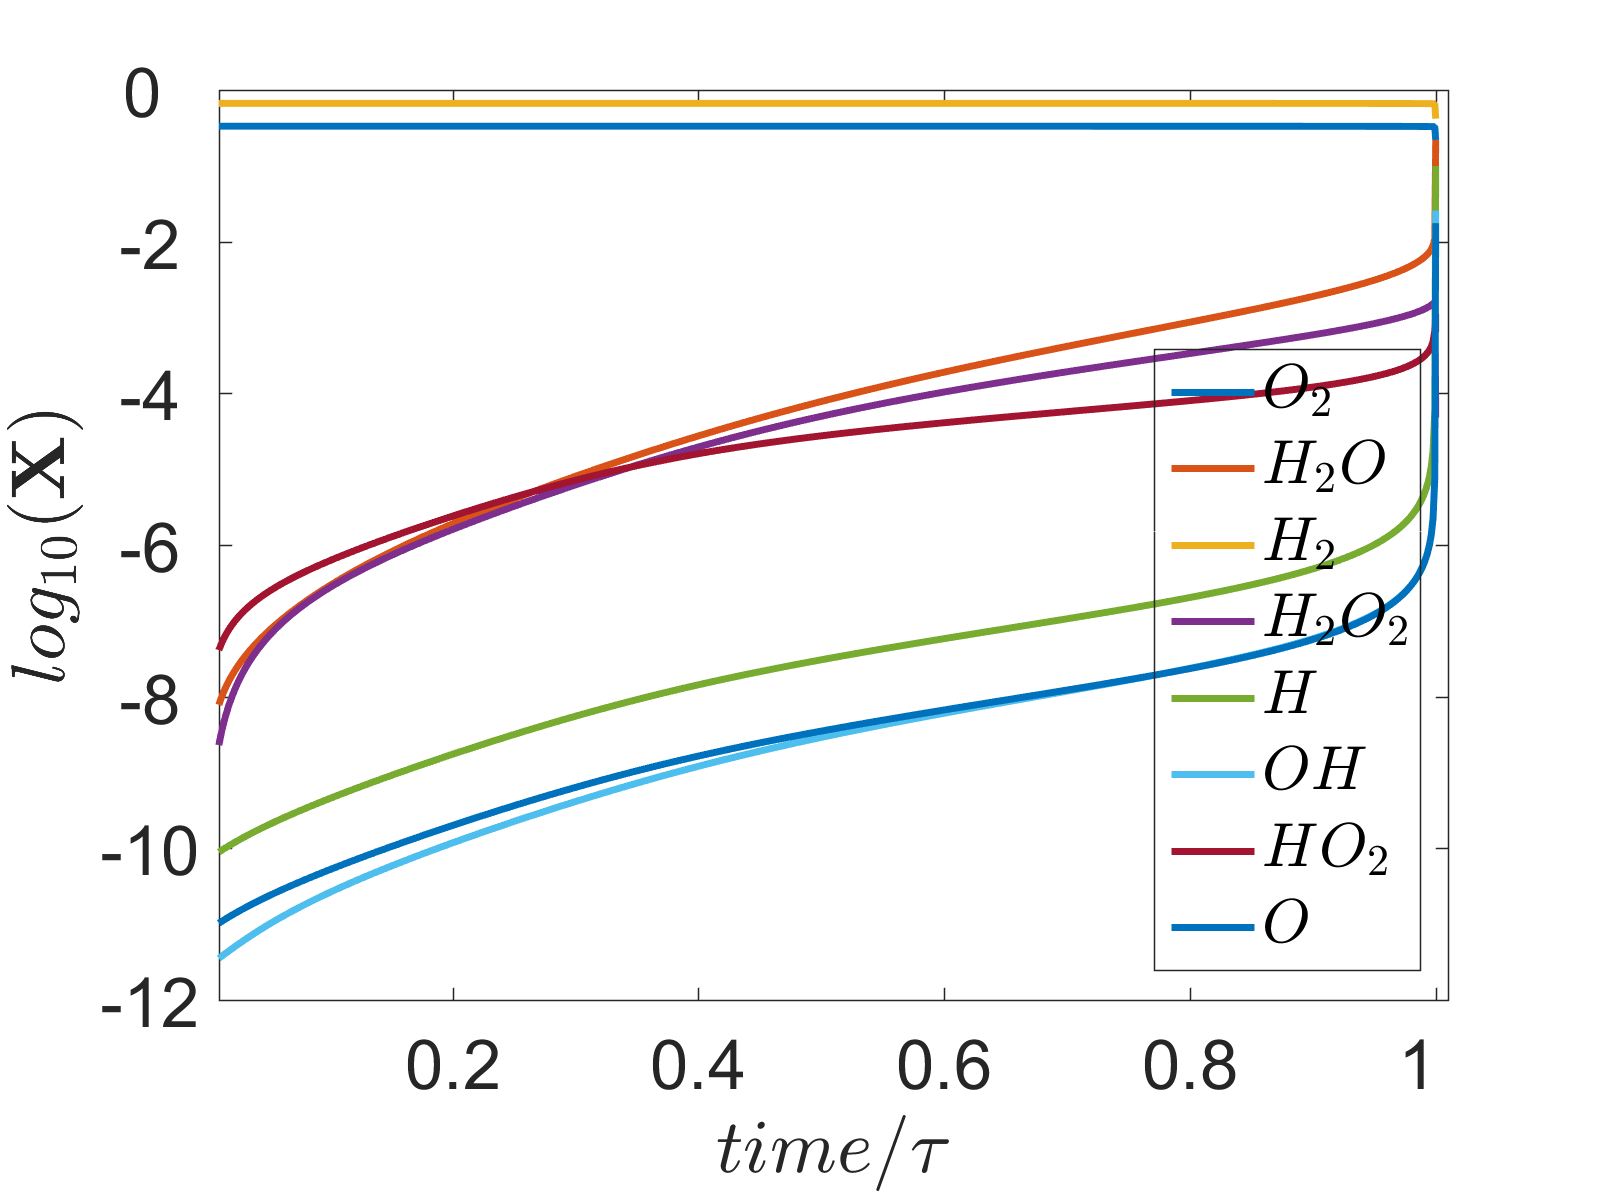
\includegraphics[width=100mm]{figs/chapter3/fig1.png}
    \end{center}
\label{ch3:fig1}
\end{figure}
\begin{figure}[htbp]
	\caption[Reaction rates versus time of H$_2$-O$_2$ combustion system]{Rates of the most important reactions versus time in units of
the ignition time. The reaction index is defined in Table \ref{ch3:spe_label} and the $\ast$ notation indicates a backward reaction.}
    \begin{center}
	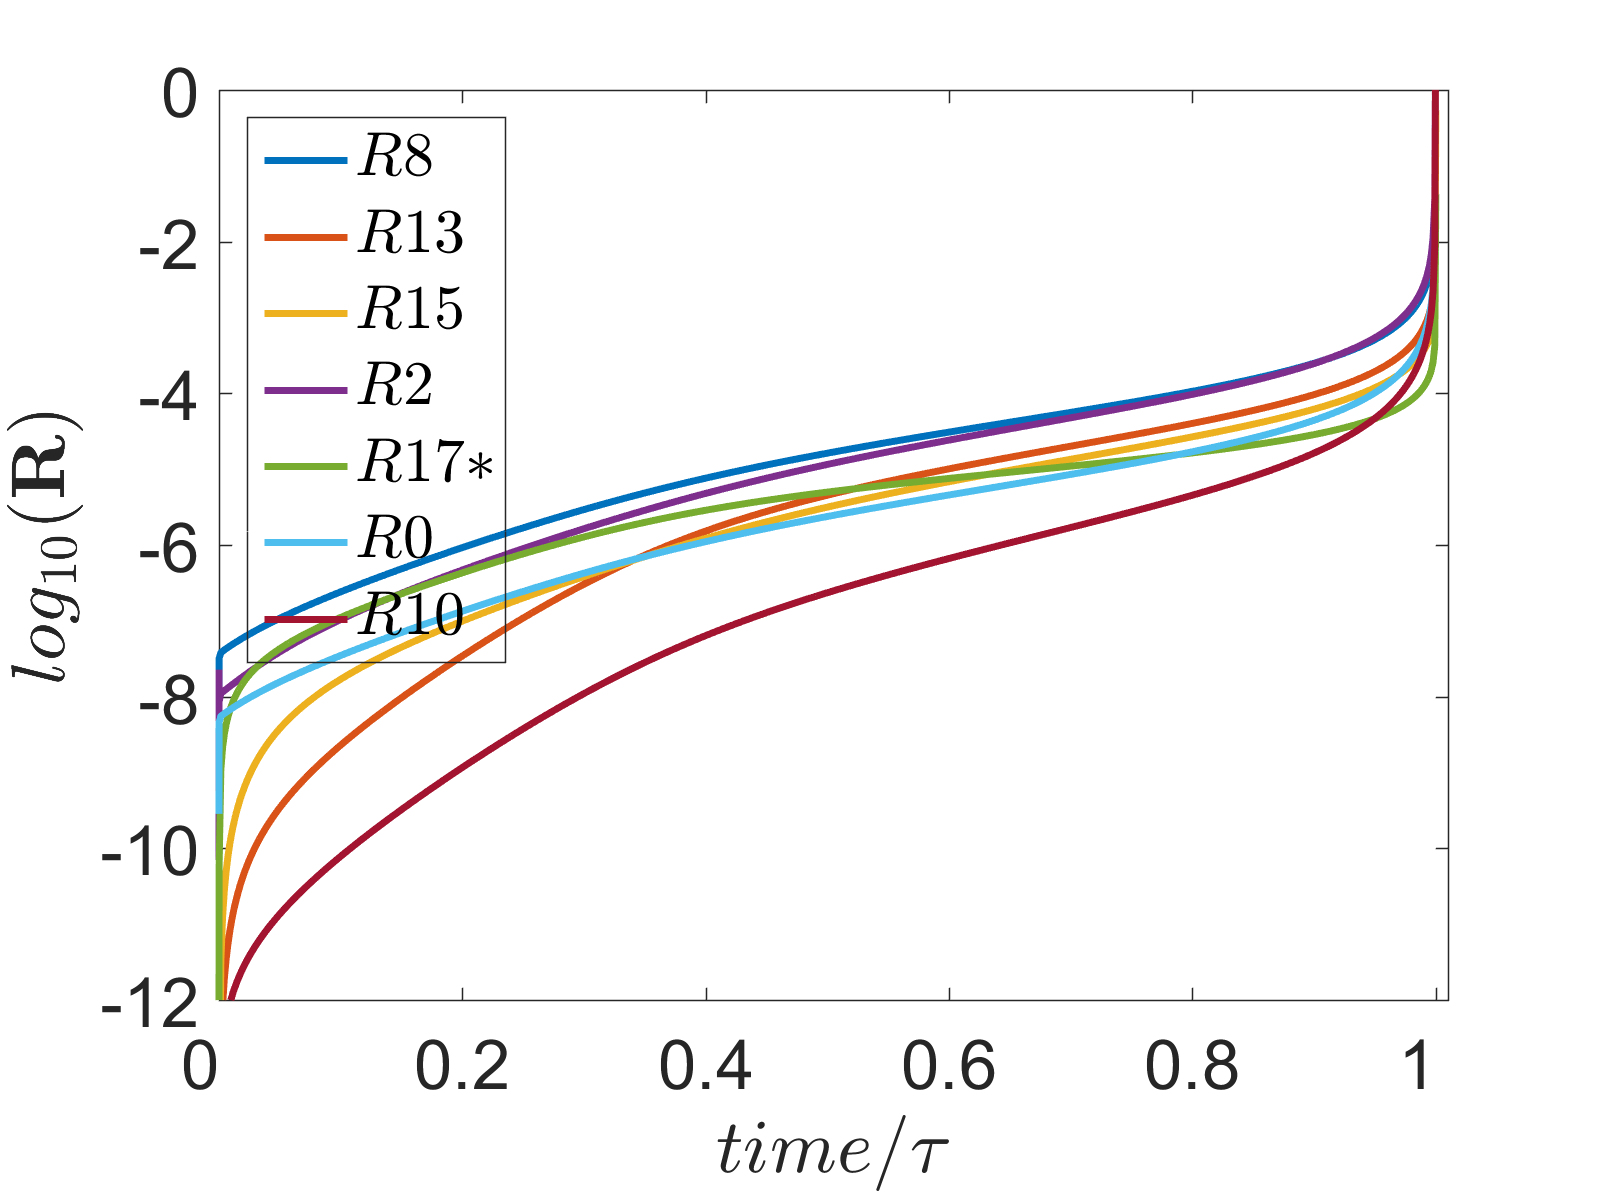
\includegraphics[width=100mm]{figs/chapter3/fig2.png}
    \end{center}
\label{ch3:fig2}
\end{figure}
\begin{figure}[htbp]
	\caption[Species decay rates versus time of H$_2$-O$_2$ combustion system]{Species decay rate, i.e., the sum of the rates of all the sink reactions, plotted versus time for all eight species.}
    \begin{center}
	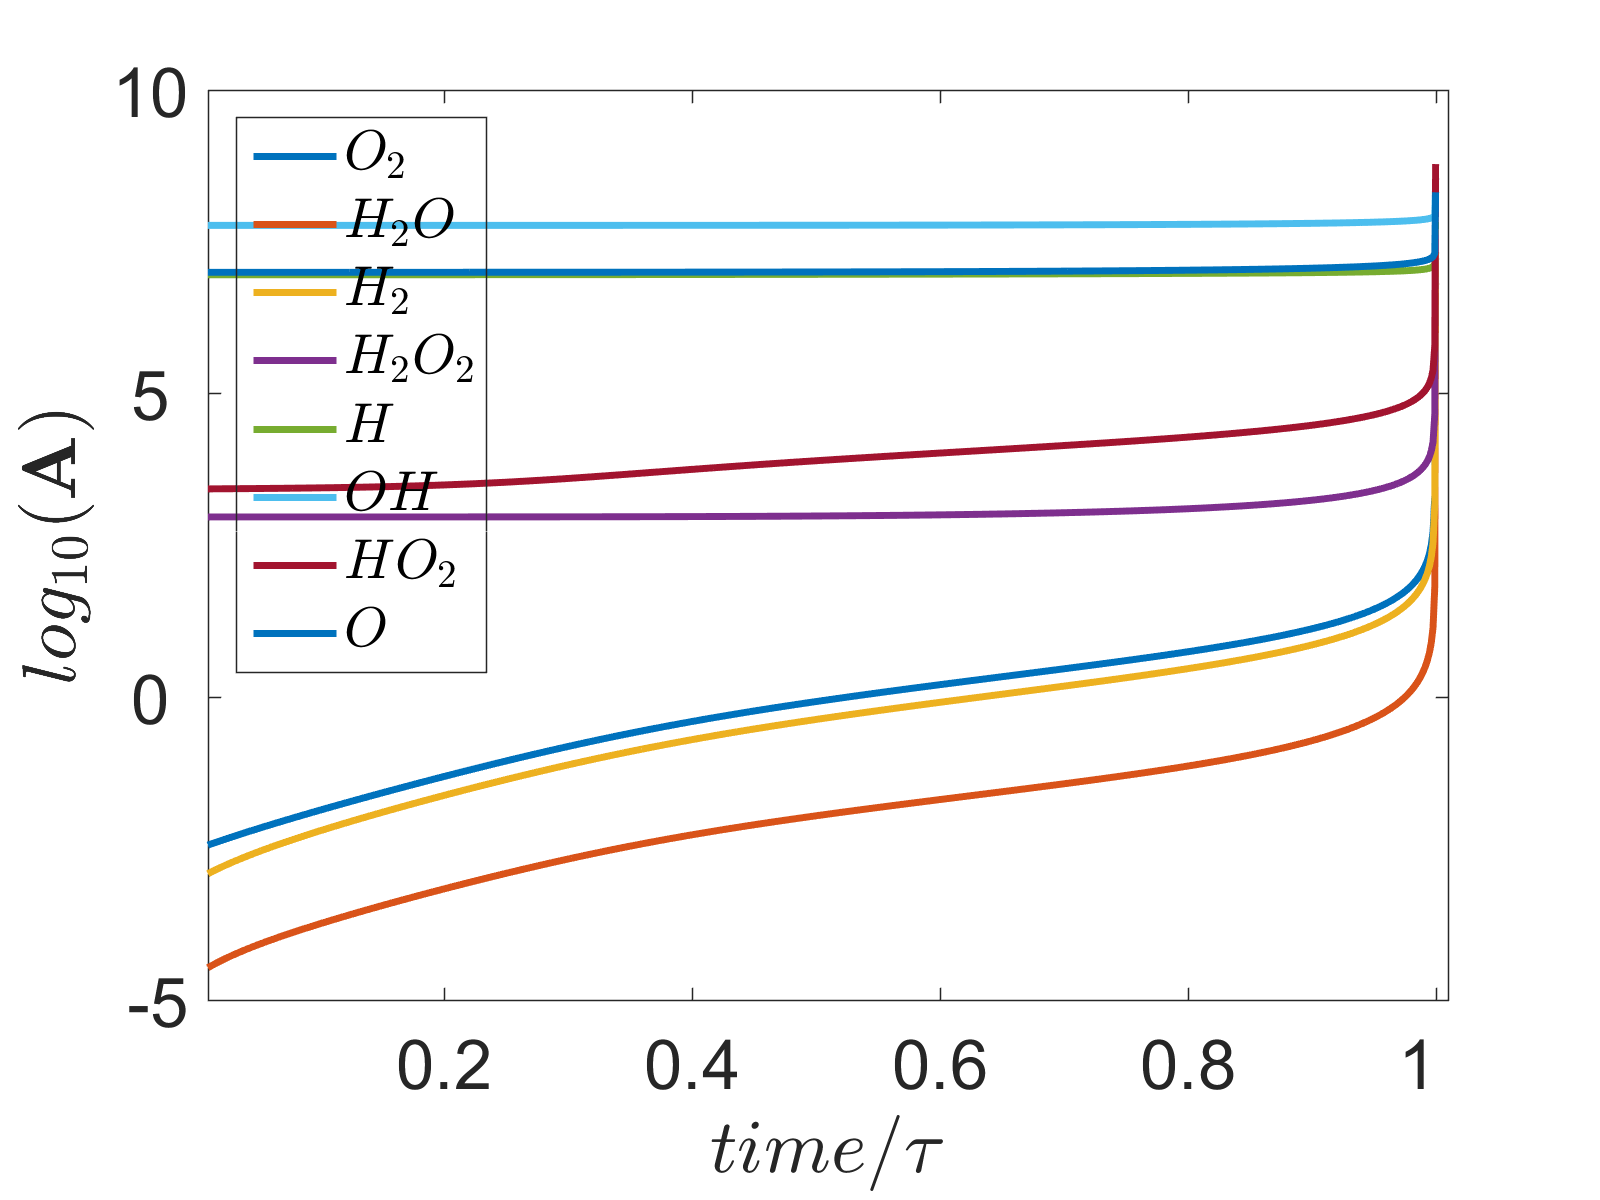
\includegraphics[width=100mm]{figs/chapter3/fig3.png}
    \end{center}
\label{ch3:fig3}
\end{figure}
The global sensitivity indices for the speciation targets $\tau=X_i(t)$ for i = 1−8 were computed at a grid of times between t =
0 and the ignition time, $\tau_{ign}$. These computations employed
numerical solutions of the kinetic rate equations, eqn. \ref{ch2:eqn2}, with
rate coefficients randomly selected from within their
uncertainty ranges. For rate coefficients of the form $k(T)=AT^{\delta}exp\left( -{E_a}/\left({RT}\right)\right)$, this sampling is accomplished by varying the value of the pre-exponential factor A. The rate coefficients
reverse reactions are set by detailed balance and thus are not
independent from the forward rates. We note that the
sensitivity index for a forward reaction, such as R17, is thus
exactly equal to that for the backward reaction, R17$\ast$, regardless
of the value of the reactive flux in the forward and backward
directions. Using 5000 sets of random rate coefficients, the
HDMR component functions $F_i(k_i)$ from eqn. \ref{ch3:eqn15:HDMR} were fit by
regression to fifth-order expansions in Legendre polynomials in
a single fitting procedure consisting of 19 $\times$ 6 = 114
parameters. As in our previous work, the sensitivity indices
were then obtained by integration using eqn. \ref{ch2:eqn16}.\cite{ch3_41_skodje2010theoretical,ch3_42_klippenstein2011uncertainty,ch3_43_davis2011global,ch3_44_zhou2013multitarget} In Fig. \ref{ch3:fig4} we show the sensitivity indices $W_i$ versus time for all 8
species. For clarity, we have included in the plot only the most
important reactions. It is seen that reactions R17, R15, R13, R9,
and R0 have consistently the highest values of $W_i$. We note that
reactions R17, R13, and R9 involve the production and
destruction of the HO$_2$ radical, which is known to play an
important role in determining the ignition properties of H$_2$ and
other fuels.\cite{ch3_46_westbrook2000chemical,ch3_47_killingsworth2011increased,ch3_48_keromnes2013experimental} Reactions R17, R15, and R13 also involve the
H$_2$O$_2$ species, which is also important in the generation of the
radical OH.\cite{ch3_49_lee1998hydrogen,ch3_50_zhou2012theoretical} Reaction R0, H + O$_2$ = OH + O, is well-known
to be a critical chain branching step in all combustion reactions.
Here, R0 is seen to be particularly important for the formation
of OH radicals. The species O is unique in being the only target
that is significantly sensitive to the reaction R1, O + H$_2$ = OH +
H.
\begin{figure}[htbp]
	\caption[Global sensitivity index $W$ versus time of H$_2$-O$_2$ combustion system]{Global sensitivity index $W$ for the speciation targets $\left[ X_i(t) \right]$ versus time. The results shown are restricted to the most sensitive reactions for each case.}
    \begin{center}
	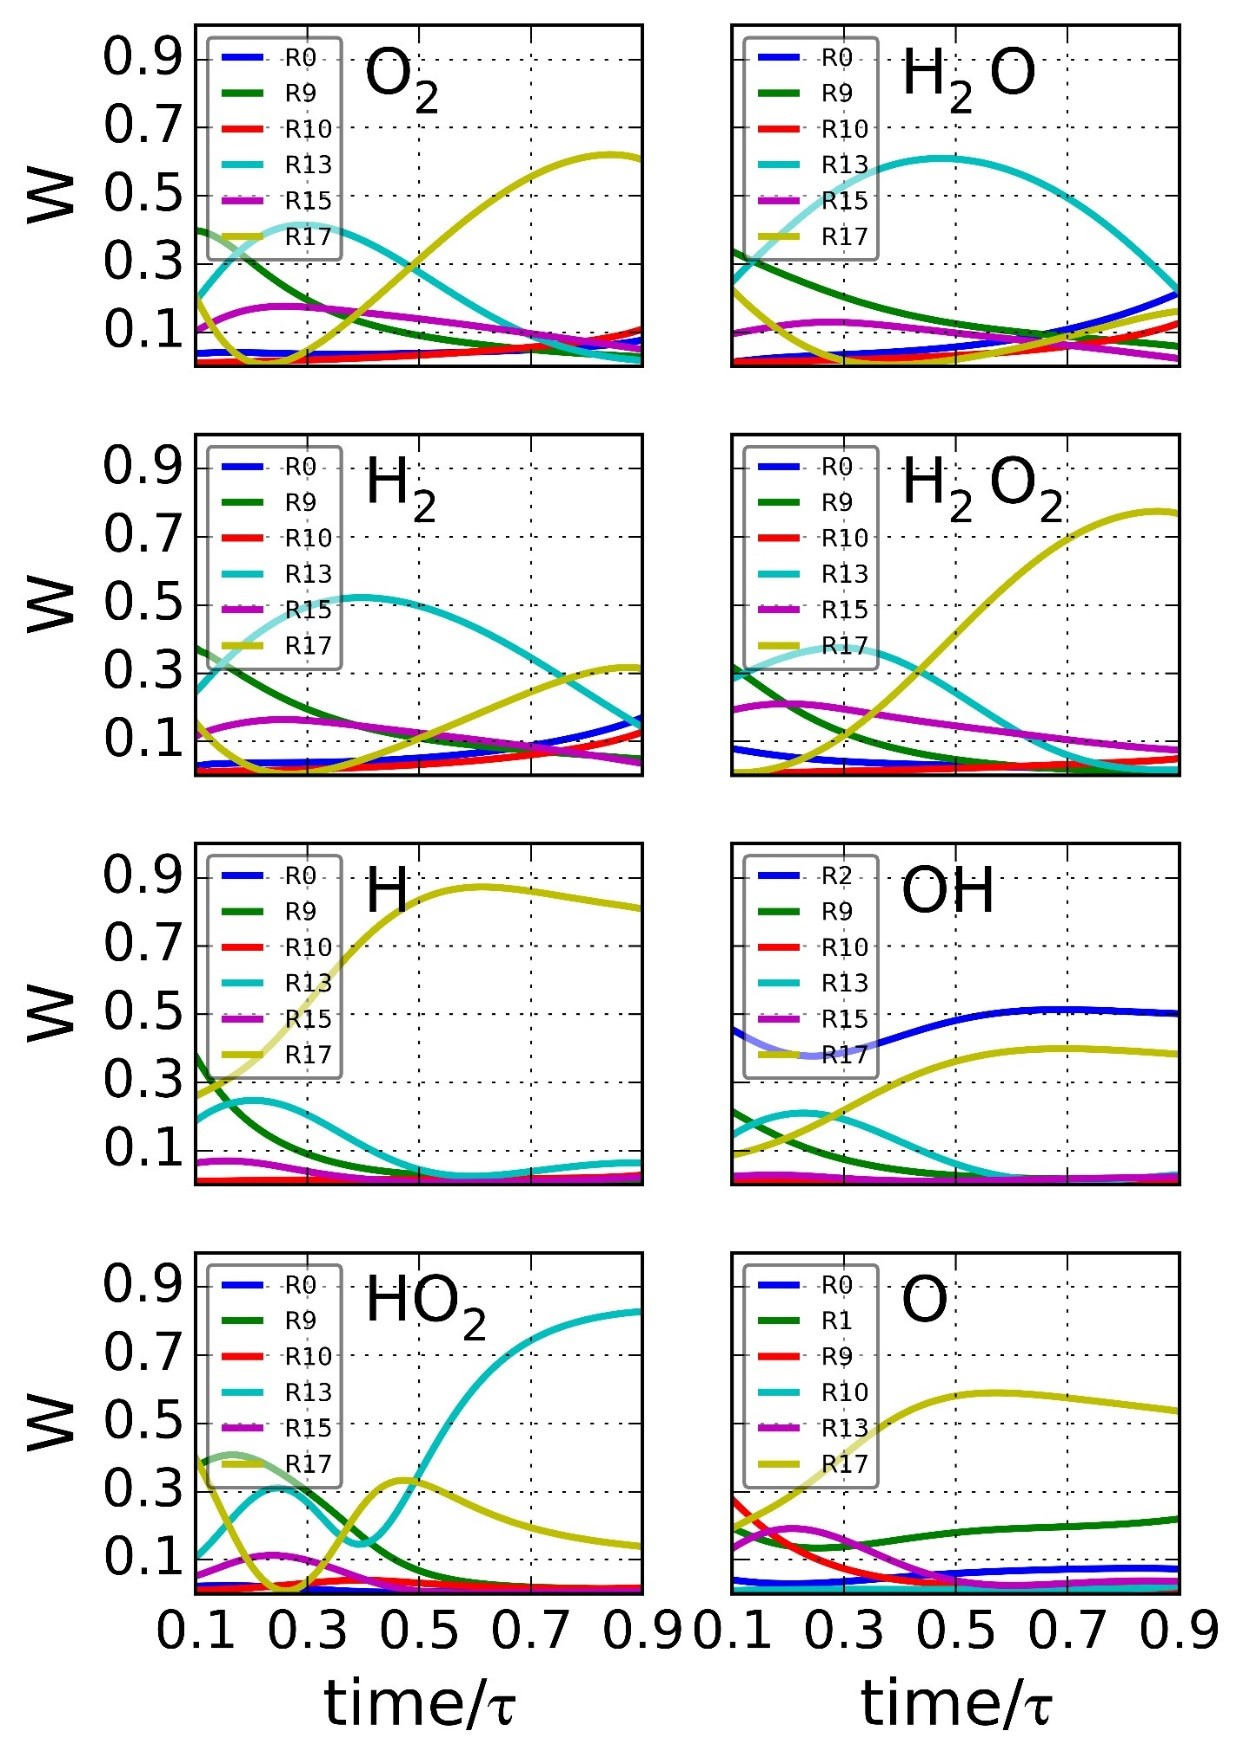
\includegraphics[width=100mm]{figs/chapter3/fig4.jpg}
    \end{center}
\label{ch3:fig4}
\end{figure}
\newline
\paragraph{}
Despite differences in the shape of the sensitivity curves for
the various species, there is actually a significant amount of
similarity in overall behavior of the results. All the species
exhibit large values at early times for the initiation reaction H$_2$ +
O$_2$ = HO$_2$ + H (R9), which then falls off sharply at later times.
This is understandable because reaction R9 is the main initiator
for autoignition but is not important for chain propagation and
chain branching. During the later stages of the reaction, $t \geq 0.4\tau_{ign}$, reactions R17 (HO$_2$ + H$_2$ = H$_2$O$_2$ + H) and R13 (HO$_2$
+ HO$_2$ = H$_2$O$_2$ + O$_2$) usually carry the largest sensitivities, as
occasionally does R15 (H$_2$O$_2$ + M = M + 2OH). It is
interesting to note for many targets we see a trend where $W_{17}$ is
more sensitive at earlier times but then is surpassed by $W_{13}$,
which grows larger at later times. For all species except H and
O, there is a crossover where $W_{17} > W_{13}$ at short times but then $W_{13} > W_{17}$ at longer times. That the sensitivity coefficients of
the different species in a large model behave similarly has been
noted previous by Skodje and Davis51 and Turanyi et al;\cite{ch3_52_zsely2005similarity} this
behavior is related to the fact that the kinetics tends to rapidly
approach a low-dimensional manifold in which the species
concentrations are slaved to one another. The equivalence
between the different sensitivity plots is only qualitative in the
present case because for global analysis the different values of
the uncertainty ranges, $\Delta k_i$, introduces quantitative differences
between the various $W_i$. This can be appreciated by noting that
global sensitivity index can be crudely approximated by $W_i \approx \left\vert \frac{d \left[ X(t) \right] }{dk_i} \times \Delta k_i \right\vert $, where $\mathbf{X}(t)$ is the species concentration
computed using the nominal (unperturbed) rate coefficients.
Thus, clearly, the relative values of $W_i$ can be adjusted using the
externally provided uncertainty ranges.

\section{Description of Chemical Pathways for H$_2$-O$_2$ Combustion}
\label{Description_of_Chemical_Pathway}
When the species target functions are expressed as linear
combinations $\tau=\sum_{i}{c_ip_i}$, the sensitivity of $\tau$ to $\mathbf{k}$ can be
understood in terms of the behavior of the pathway
probabilities. Hence, we must first determine a sufficient
number of chemical pathways and their probabilities to
converge the speciation targets of interest, $ X_i(t)$. Then, we
investigate the $\mathbf{k}$ dependence of the probabilities. In our
previous work, we studied the early stage combustion of
hydrogen using an H atom following scheme. It was found that convergence of the concentrations to within several percent was
obtained using about a dozen chemical pathways. Here, we reexamine
the pathway representation using, instead, O atom
following pathways. Although convergence to the exact result
may be obtained by following any moiety present in the target
species, the choice of followed atom may affect the efficiency of
the algorithm. In the present case, we find that O atom
following converges significantly faster than H atom following.
For reference, in Fig. \ref{ch3:fig5} we show the full graph that shows all species (nodes) and the most important reactions (lines) that
contribute to the present mechanism. The O atom following
pathways lie on the subgraph containing only the oxygen
possessing species.
\begin{figure}[htbp]
	\caption[Oxygen subgraph of H$_2$-O$_2$ combustion system]{Graph representing all species and the most important reactions for the H$_2$-O$_2$ system by following Oxygen atom.}
    \begin{center}
	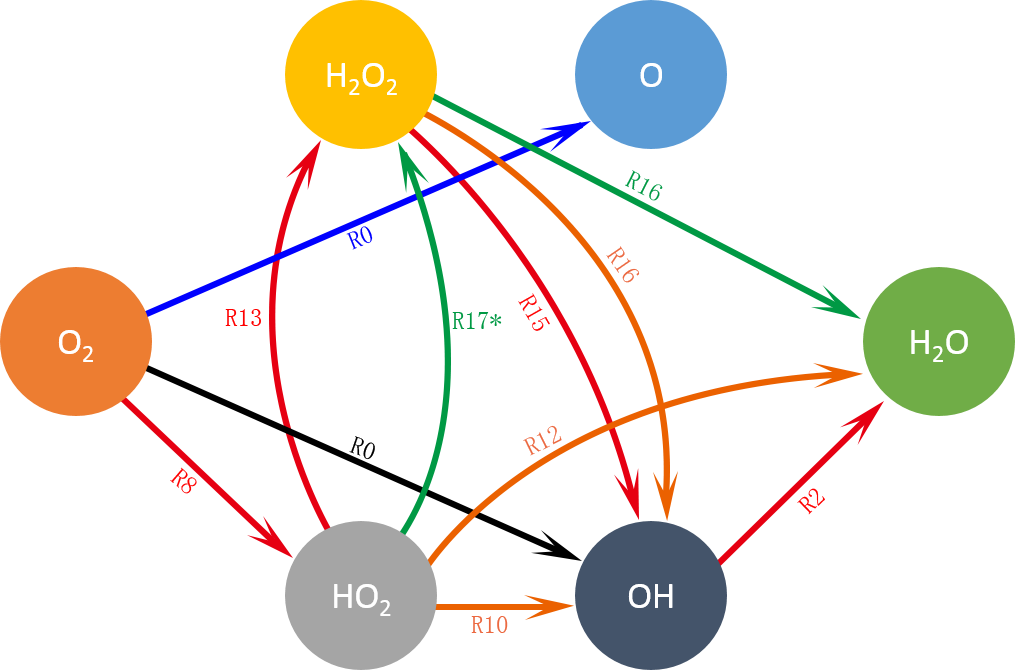
\includegraphics[width=100mm]{figs/chapter3/fig5.png}
    \end{center}
\label{ch3:fig5}
\end{figure}
\newline
\paragraph{}
To identify a set of “candidate” pathways for study, we first
use a small size stochastic simulation, i.e., $10^5-10^6$ simulated
paths, computed at the nominal value of $\mathbf{k}$. Thus, during a time
interval $\Delta t$, a given molecule of $S_i$ has a decay probability of
$A_i(t) \Delta t$. Using one random number to sample this decay, and a
second random number to select a product branch $j$, $\Gamma_j(t)$, a
given O atom is then followed through the network one node
(species) at a time. Recording each pathway that occurs, an
approximately ordered set of candidates is produced that
describes the passage of a followed atom to a given target. For
the present problem, typically about 100 pathways were
identified in this way, although many fewer were needed to
converge the targets. Although this calculation is not efficient
enough to compute accurate pathway probabilities, it does yield
the important pathways for high level computation using eqn. \ref{ch2:eqn13}
or \ref{ch2:eqn14}. Because the ordering of the pathway probabilities will be
a function of $\mathbf{k}$, we retain some of the smaller probability
pathways because they may become larger in certain regions of
k-space.
\newline
\paragraph{}
\begin{figure}[htbp]
	\caption[Pathway probabilities for H$_2$O$_2$ of H$_2$-O$_2$ combustion system]{Pathway probabilities for H$_2$O$_2$. In the upper panel, the probabilities for the five most important pathways, ranked at time $t=0.8\tau_{ign}$, are shown versus time in units of $\tau$. In the middle panel, the same probabilities are reproduced on a logarithmic scale. In the lower panel, the convergence of the concentration to the “exact” simulation result is shown; it is seen that probability converges to good accuracy
with just two paths.}
    \begin{center}
	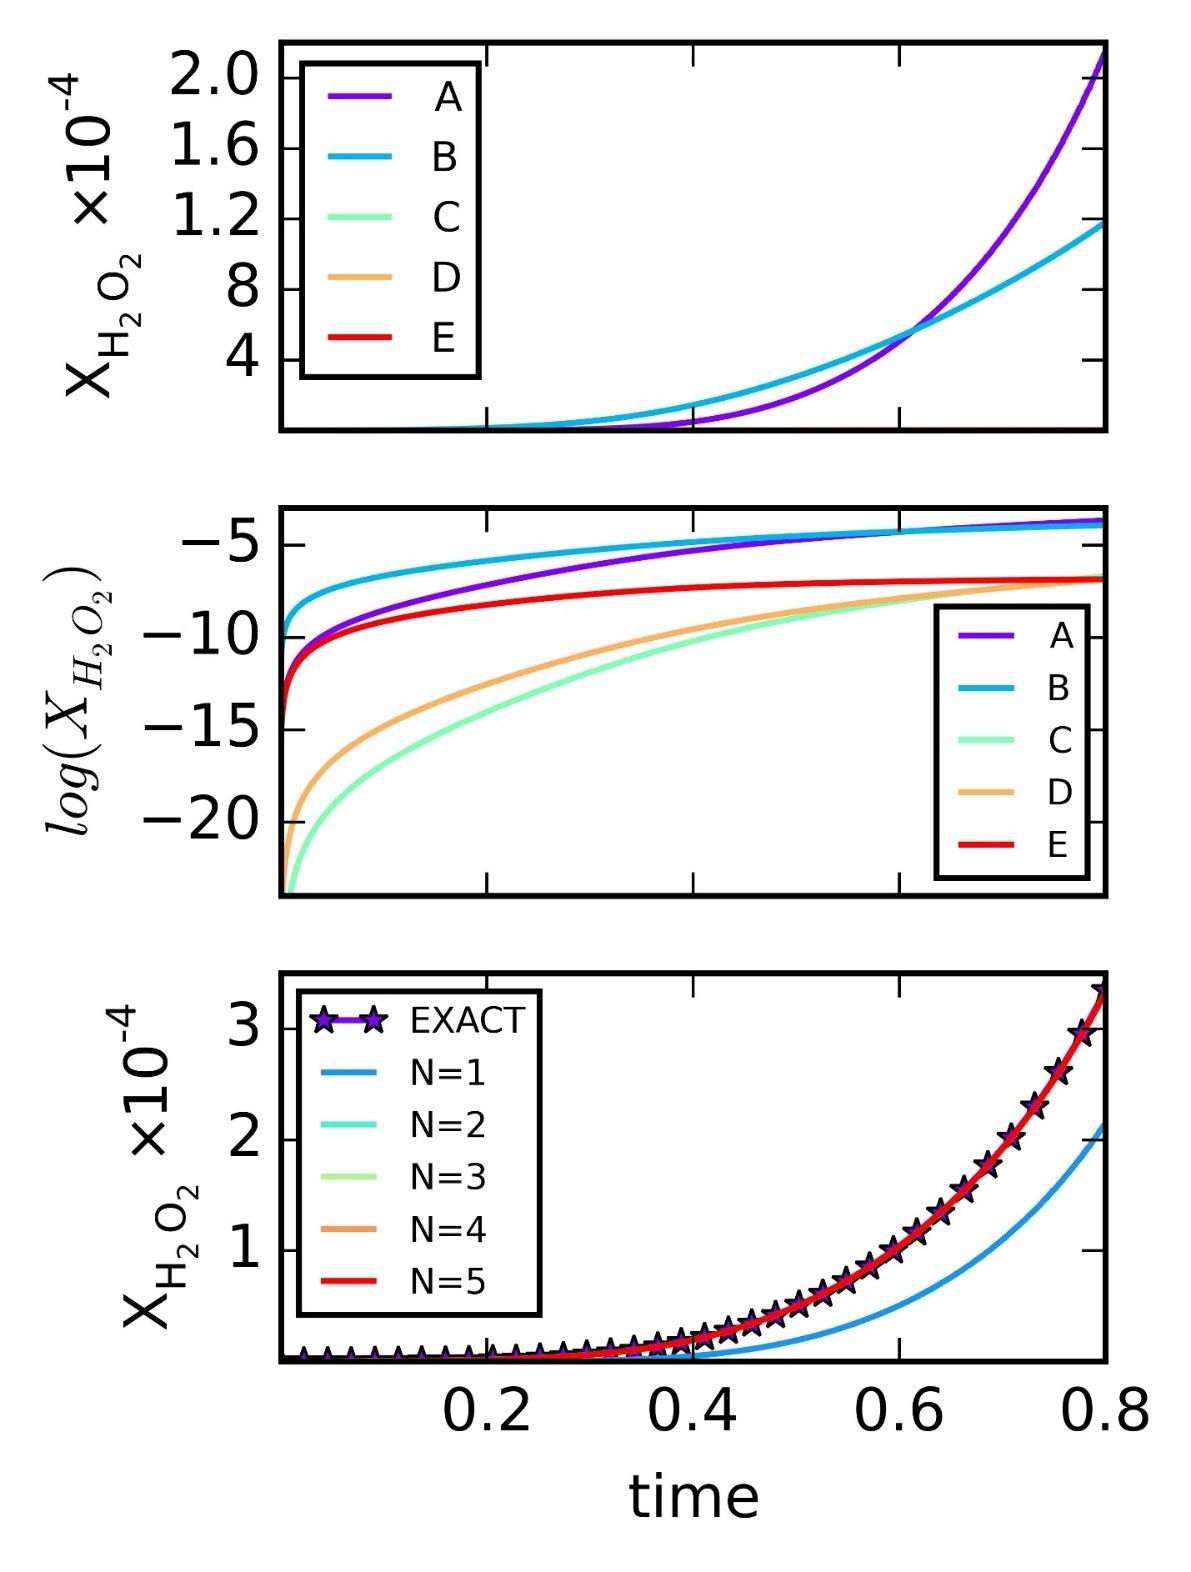
\includegraphics[width=100mm]{figs/chapter3/fig6.jpg}
    \end{center}
\label{ch3:fig6}
\end{figure}
We begin by showing the most probable pathways for the
creation of several important target species. Consider first the
formation of the transient intermediate H$_2$O$_2$ which was used
as a test case in our previous work. Although we see from Table
\ref{ch3:rxn_label} that there are six elementary reactions that generate H$_2$O$_2$, we
find that just two chemical pathways are sufficient to converge
$\left[\textrm{H}_2\textrm{O}_2\right]$ to within 1\% at times in the range $0 < t < 0.9\tau_{ign}$. In
Fig. \ref{ch3:fig6} we show the pathway probabilities for these paths,
along with the prediction for $\left[\textrm{H}_2\textrm{O}_2 (t) \right]$. Many more paths were
required to converge the results using the H atom following
algorithm. The two dominate chemical pathways for the
formation of this species are path a3 (where “a” means the most probable pathway and “3” indicates that H$_2$O$_2$ is species 3 in
Table \ref{ch3:spe_label})
%\begin{equation*}
%\label{ch3:path:a3}
%\tag{a3}
%haha
%\end{equation*}
%The & sign separates two columns, so an & at the beginning of a line means that the line starts with a blank column.
%https://stackoverflow.com/questions/2632628/left-align-block-of-equations
\begin{flalign*}
\label{ch3:path:a3}
\tag{a3}
	&\textcolor{red}{\textbf{O}}_2(+\text{H}+\text{M}) \xrightarrow[\text{R}_8]{\makebox[1cm]{}} \text{H}\textcolor{red}{\textbf{O}}_2(+\text{H}\text{O}_2) \xrightarrow[\text{R}_{13}]{\makebox[1cm]{}} \text{H}_2\textcolor{red}{\textbf{O}}_2 &
\end{flalign*}
and path b3 (“b” for the second most probable pathway, etc.)
\begin{flalign*}
\label{ch3:path:b3}
\tag{b3}
	&\textcolor{red}{\textbf{O}}_2(+\text{H}+\text{M}) \xrightarrow[\text{R}_8]{\makebox[1cm]{}} \text{H}\textcolor{red}{\textbf{O}}_2(+\text{H}_2) \xrightarrow[\text{R}_{17}^{\ast}]{\makebox[1cm]{}} \text{H}_2\textcolor{red}{\textbf{O}}_2 &
\end{flalign*}
In the chemical pathway formulas, we indicated the followed
atom in red, the nonfollowed reagents are in parentheses, and
the nonfollowed products are dropped from the equation. We
can see by the figure that the pathway probabilities for H$_2$O$_2$
formation show a crossover behavior where the path involving
R17$^\ast$ is largest at short times whereas the path containing R13
is larger at long times. The remaining pathways we computed
were lower in probability by factors of 100 or more. The next
three pathways are
\begin{flalign*}
\label{ch3:path:c3}
\tag{c3}
	&\textcolor{red}{\textbf{O}}_2(+\text{H}+\text{M}) \xrightarrow[\text{R}_8]{\makebox[1cm]{}} \text{H}\textcolor{red}{\textbf{O}}_2(+\text{H}\text{O}_2) \xrightarrow[\text{R}_{13}]{\makebox[1cm]{}} \text{H}_2\textcolor{red}{\textbf{O}}_2 (+ \text{H}) \xrightarrow[\text{R}_{17}]{\makebox[1cm]{}} \text{H}\textcolor{red}{\textbf{O}}_2(+\text{H}\text{O}_2) \xrightarrow[\text{R}_{13}]{\makebox[1cm]{}} \text{H}_2\textcolor{red}{\textbf{O}}_2 &
\end{flalign*}
\begin{flalign*}
\label{ch3:path:d3}
\tag{d3}
	&\textcolor{red}{\textbf{O}}_2(+\text{H}_2) \xrightarrow[\text{R}_9^{\ast}]{\makebox[1cm]{}} \text{H}\textcolor{red}{\textbf{O}}_2(+\text{H}\text{O}_2) \xrightarrow[\text{R}_{13}]{\makebox[1cm]{}} \text{H}_2\textcolor{red}{\textbf{O}}_2 &
\end{flalign*}
\begin{flalign*}
\label{ch3:path:e3}
\tag{e3}
	&\textcolor{red}{\textbf{O}}_2(+\text{H}+\text{M}) \xrightarrow[\text{R}_8]{\makebox[1cm]{}} \text{H}\textcolor{red}{\textbf{O}}_2(+\text{H}_2) \xrightarrow[\text{R}_{17}^{\ast}]{\makebox[1cm]{}} \text{H}_2\textcolor{red}{\textbf{O}}_2 (+ \text{H}) \xrightarrow[\text{R}_{17}]{\makebox[1cm]{}} \text{H}\textcolor{red}{\textbf{O}}_2(+\text{H}\text{O}_2) \xrightarrow[\text{R}_{13}]{\makebox[1cm]{}} \text{H}_2\textcolor{red}{\textbf{O}}_2 &
\end{flalign*}
%\newline
\paragraph{}
It is interesting to note that pathways c3 and e3 are quite closely related to the main pathways a3 and b3. We see that in mechanism c3, the H$_2$O$_2$ is formed along pathway a3 but then is recycled back to HO$_2$ by H atom attack,
, only then to regenerate H$_2$O$_2$ by radical−radical recombination, R13. In mechanism e3, we see
the same scenario except the initial H$_2$O$_2$ molecule is generated
by path b3. In mechanism d3, the H$_2$O$_2$ is formed by radical
recombination R13 but the followed species HO$_2$ is generated
by the initiation reaction R9, i.e., H$_2$+ O$_2$ $\rightarrow$ HO$_2$ + H rather
the higher flux reaction R6. For reference, we indicate the
contributing pathways on the O atom subgraph in Fig. \ref{ch3:fig7}.
\begin{figure}[htbp]
	\caption[Graph for the oxygen following paths of H$_2$-O$_2$ combustion system]{Graph for the oxygen following paths, a3 - e3, leading to the H$_2$O$_2$ product.}
    \begin{center}
	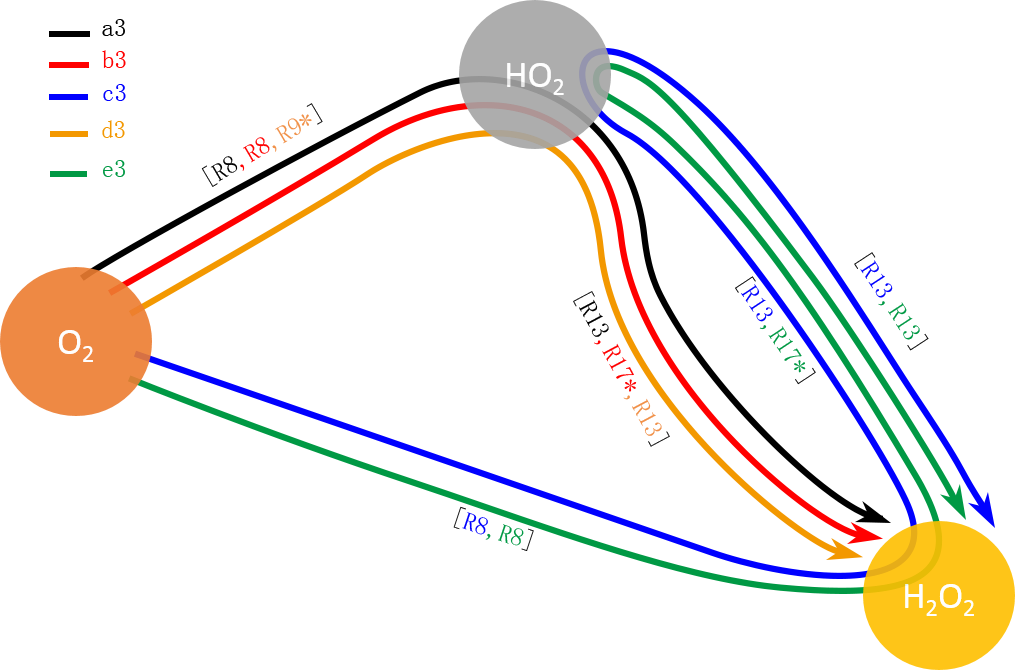
\includegraphics[width=100mm]{figs/chapter3/fig7.png}
    \end{center}
\label{ch3:fig7}
\end{figure}
\begin{figure}[htbp]
	\caption[Pathway probabilities for H$_2$O of H$_2$-O$_2$ combustion system]{Same as Fig. \ref{ch3:fig6} except for the target function $\left[ \text{H}_2\text{O}(t) \right]$.}
    \begin{center}
	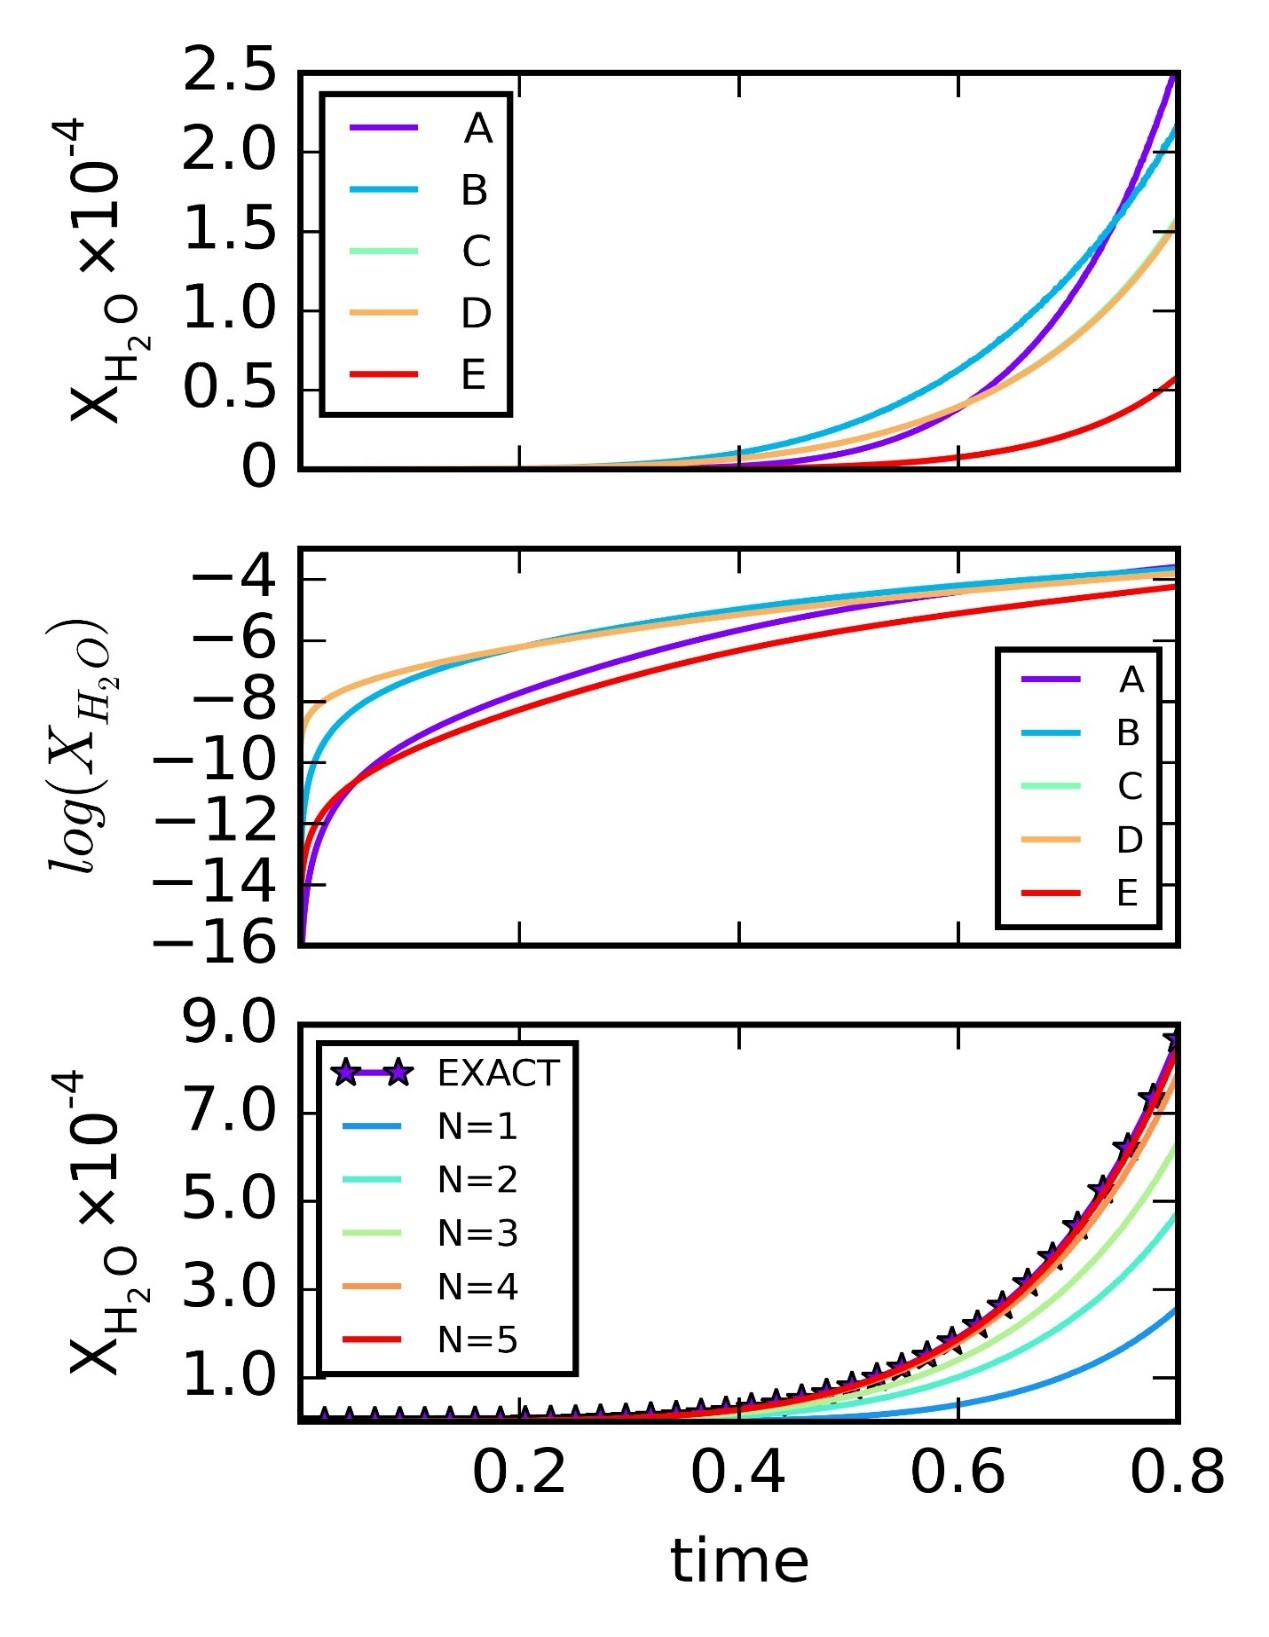
\includegraphics[width=100mm]{figs/chapter3/fig8.jpg}
    \end{center}
\label{ch3:fig8}
\end{figure}
\paragraph{}
\newline
\paragraph{}
For the H$_2$O product species (species 1 in Table \ref{ch3:spe_label}), we find
that there are more contributing pathways than for H$_2$O$_2$. We find that five paths account for about 98% of the H$_2$O
formation under the present conditions. The convergence of
the target $\left[\text{H}_2\text{O}(t)\right]$ versus time is shown in Fig. \ref{ch3:fig8}. The most
important O atom following pathways that connect the O$_2$
reagent to the H$_2$O product are
\begin{flalign*}
\label{ch3:path:a1}
\tag{a1}
	&\textcolor{red}{\textbf{O}}_2(+\text{H}+\text{M}) \xrightarrow[\text{R}_8]{\makebox[1cm]{}} \text{H}\textcolor{red}{\textbf{O}}_2(+\text{H}\text{O}_2) \xrightarrow[\text{R}_{13}]{\makebox[1cm]{}} \text{H}_2\textcolor{red}{\textbf{O}}_2 (+ \text{M}) \xrightarrow[\text{R}_{15}]{\makebox[1cm]{}} \textcolor{red}{\textbf{O}}\text{H}(+\text{H}_2) \xrightarrow[\text{R}_{2}]{\makebox[1cm]{}} \text{H}_2\textcolor{red}{\textbf{O}} &
\end{flalign*}
\begin{flalign*}
\label{ch3:path:b1}
\tag{b1}
	&\textcolor{red}{\textbf{O}}_2(+\text{H}+\text{M}) \xrightarrow[\text{R}_8]{\makebox[1cm]{}} \text{H}\textcolor{red}{\textbf{O}}_2(+\text{H}_2) \xrightarrow[\text{R}_{17}^{\ast}]{\makebox[1cm]{}} \text{H}_2\textcolor{red}{\textbf{O}}_2 (+ \text{M}) \xrightarrow[\text{R}_{15}]{\makebox[1cm]{}} \textcolor{red}{\textbf{O}}\text{H}(+\text{H}_2) \xrightarrow[\text{R}_{2}]{\makebox[1cm]{}} \text{H}_2\textcolor{red}{\textbf{O}} &
\end{flalign*}
\begin{flalign*}
\label{ch3:path:c1}
\tag{c1}
	&\textcolor{red}{\textbf{O}}_2 (+ \text{H}) \xrightarrow[\text{R}_{0}]{\makebox[1cm]{}} \textcolor{red}{\textbf{O}}\text{H}(+\text{H}_2) \xrightarrow[\text{R}_{2}]{\makebox[1cm]{}} \text{H}_2\textcolor{red}{\textbf{O}} &
\end{flalign*}
\begin{flalign*}
\label{ch3:path:d1}
\tag{d1}
	&\textcolor{red}{\textbf{O}}_2 (+ \text{H}) \xrightarrow[\text{R}_{0}]{\makebox[1cm]{}} \textcolor{red}{\textbf{O}} (+ \text{H}_2)  \xrightarrow[\text{R}_{1}]{\makebox[1cm]{}} \textcolor{red}{\textbf{O}}\text{H}(+\text{H}_2) \xrightarrow[\text{R}_{2}]{\makebox[1cm]{}} \text{H}_2\textcolor{red}{\textbf{O}} &
\end{flalign*}
\begin{flalign*}
\label{ch3:path:e1}
\tag{e1}
	&\textcolor{red}{\textbf{O}}_2 (+ \text{H}+\text{M}) \xrightarrow[\text{R}_{8}]{\makebox[1cm]{}} \text{H}\textcolor{red}{\textbf{O}}_2 (+ \text{H})  \xrightarrow[\text{R}_{10}]{\makebox[1cm]{}} \textcolor{red}{\textbf{O}}\text{H}(+\text{H}_2) \xrightarrow[\text{R}_{2}]{\makebox[1cm]{}} \text{H}_2\textcolor{red}{\textbf{O}} &
\end{flalign*}
\newline
\paragraph{}
The two most probable pathways, a1 and b1, again generate
an H$_2$O$_2$ intermediate from HO$_2$ radicals, which indicates that a
large fraction of the H$_2$O product passes through this
intermediate species. Indeed, the first three steps for a1 and
b1 are seen to be identical to the dominate pathways for H$_2$O$_2$
formation, i.e., a3 and b3. In both a1 and b1, the H$_2$O$_2$ breaks
down via the unimolecular dissociation reaction R15 with the
resulting OH radical converted to water through the reaction
R2, i.e., OH + H$_2$ $\rightarrow$ H$_2$O + H. From the figure, we again note a crossover behavior where path a1 (containing R13) is more
probable at long times whereas path b1 (contain R17*) is more
probable at shorter times. The three next most probable
pathways are mechanistically distinct from the H$_2$O$_2$ forming
pathways a1 and b1. It is seen in Fig. \ref{ch3:fig8} that the contributions
from c1 and d1 are nearly identical because it is clear that these
paths are closely related. In these two pathways, we are tracking
the separate progress of the two oxygen atoms of O$_2$ following
the initiation reaction R0, i.e., O$_2$ + H $\rightarrow$ OH + O. In the first
case, c1, the OH radical from R0 reacts quickly with H$_2$ to
produce the water product in a single step, R2. Along the other
path, d1, the O atom product of R0 first abstracts an H atom
via R1 to form OH and then the OH reacts with H$_2$ to form
water. Because nearly all the OH is consumed to form H$_2$O and
nearly all the O reacts with H$_2$ to form OH, it is not surprising
that the probabilities for c3 and d3 are very close. In both cases,
the species containing the followed O atom quickly forms water
upon reaction with H$_2$. Finally, pathway e5 again is initiated by
formation of HO$_2$ through the recombination reaction R8.
However, in e5 the HO$_2$ radical reacts with H via R10 to form
the OH radical, which then quickly converts to H$_2$O by R10.
The five pathways are depicted graphically in Fig. \ref{ch3:fig9}.
\newline
\paragraph{}
Finally, we consider the speciation of the critical HO$_2$ radical.
In Fig. \ref{ch3:fig10}, we show the relevant pathway probabilities for of
the $\left[\text{HO}_2(t)\right]$. It is very interesting to note that one pathway
carries the vast majority of the probability. Specifically, almost
all of the HO$_2$ species is generated by the recombination mechanism
\begin{flalign*}
\label{ch3:path:a6}
\tag{a6}
	&\textcolor{red}{\textbf{O}}_2 (+ \text{H}+\text{M}) \xrightarrow[\text{R}_{8}]{\makebox[1cm]{}} \text{H}\textcolor{red}{\textbf{O}}_2 &
\end{flalign*}
\begin{figure}[htbp]
	\caption[Oxygen atom following pathways leading to the formation of the H$_2$O product]{Oxygen atom following pathways leading to the formation of the H$_2$O product.}
    \begin{center}
	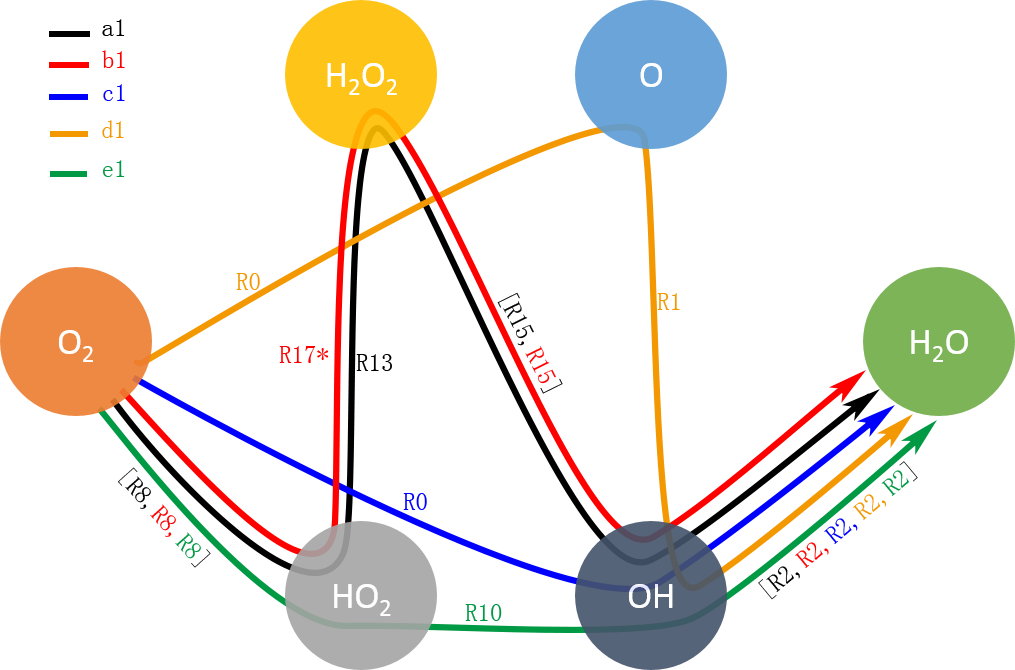
\includegraphics[width=100mm]{figs/chapter3/fig9.png}
    \end{center}
\label{ch3:fig9}
\end{figure}
\begin{figure}[htbp]
	\caption[Pathway probabilities for HO$_2$ of H$_2$-O$_2$ combustion system]{Same as Fig. \ref{ch3:fig6} except for the HO$_2$ product.}
    \begin{center}
	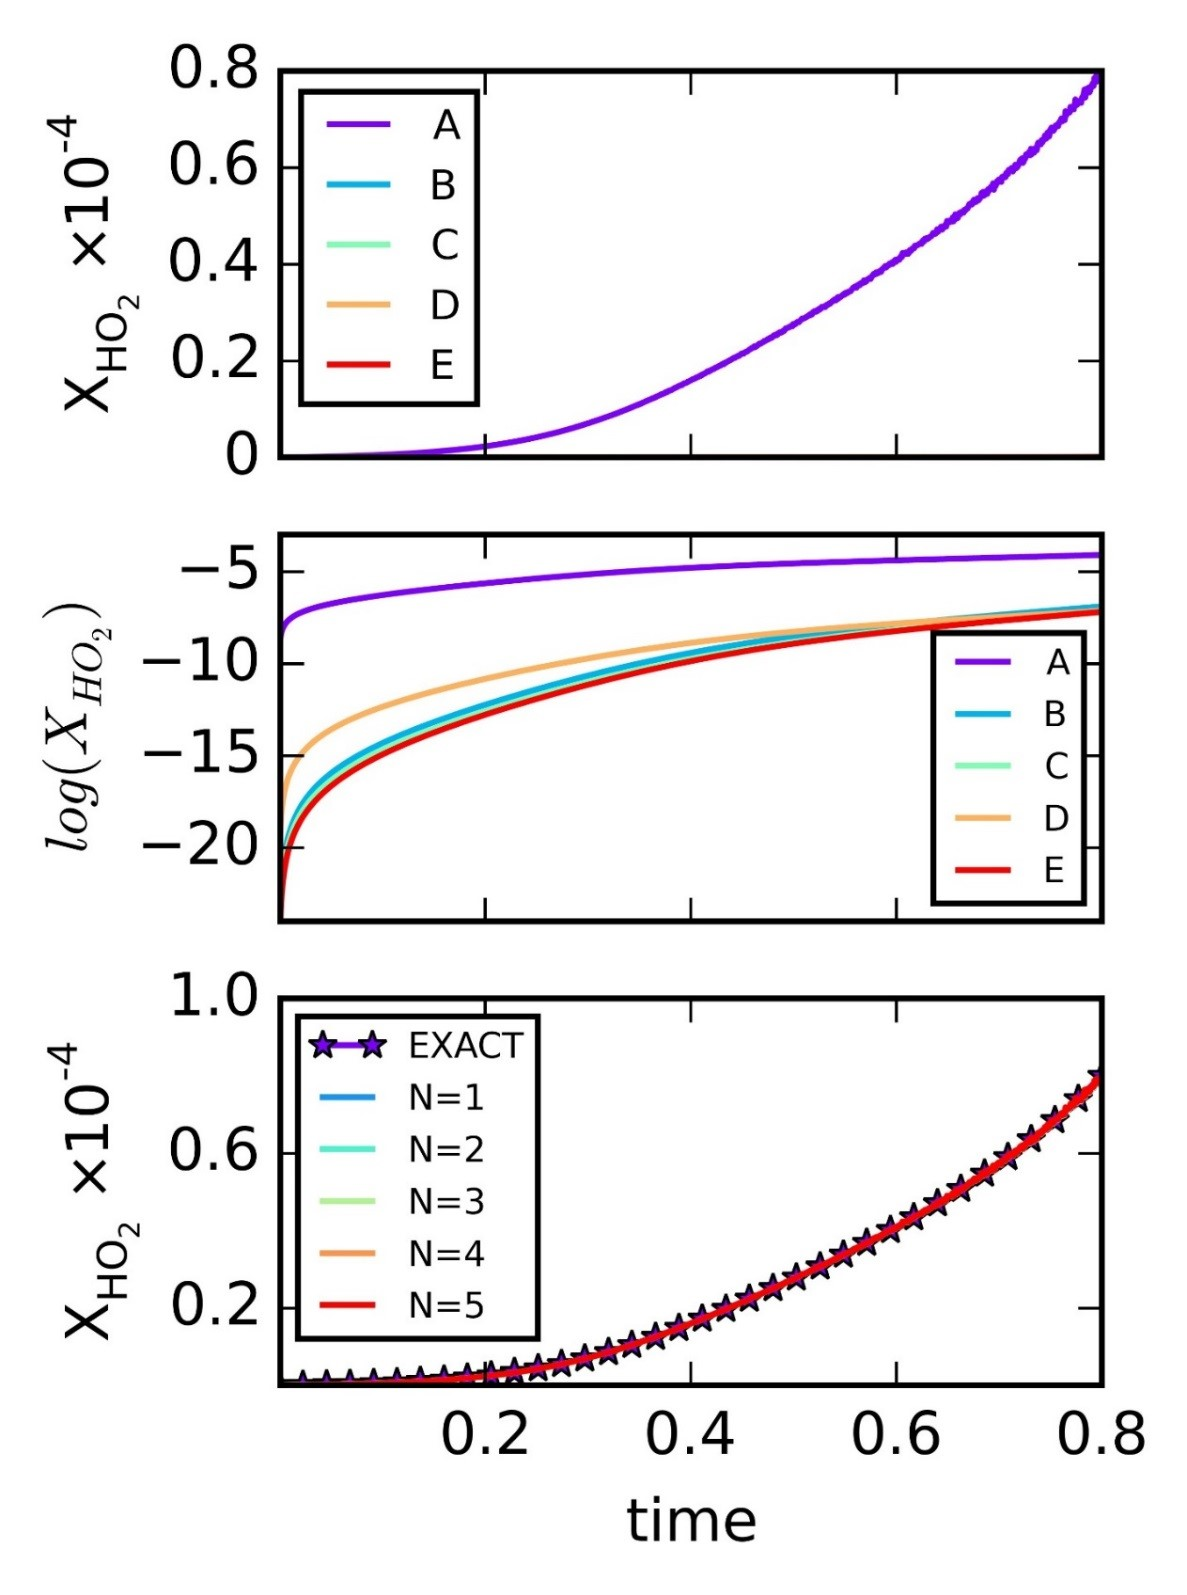
\includegraphics[width=100mm]{figs/chapter3/fig10.jpg}
    \end{center}
\label{ch3:fig10}
\end{figure}
As seen in the figure, the probabilities for other production
pathways are lower by at least a factor of 1000. For
completeness, however, we note that the algorithm does
quantify the probabilities for the other minor pathways
\begin{flalign*}
\label{ch3:path:b6}
\tag{b6}
	&\textcolor{red}{\textbf{O}}_2 (+ \text{H}+\text{M}) \xrightarrow[\text{R}_{8}]{\makebox[1cm]{}} \text{H}\textcolor{red}{\textbf{O}}_2 (+\text{HO}_2) \xrightarrow[\text{R}_{13}]{\makebox[1cm]{}} \text{H}_2\textcolor{red}{\textbf{O}}_2 (+\text{H}) \xrightarrow[\text{R}_{17}]{\makebox[1cm]{}} \text{H}\textcolor{red}{\textbf{O}}_2 &
\end{flalign*}
\begin{flalign*}
\label{ch3:path:c6}
\tag{c6}
	&\textcolor{red}{\textbf{O}}_2 (+ \text{H}+\text{M}) \xrightarrow[\text{R}_{8}]{\makebox[1cm]{}} \text{H}\textcolor{red}{\textbf{O}}_2 (+\text{HO}_2) \xrightarrow[\text{R}_{13}]{\makebox[1cm]{}} \textcolor{red}{\textbf{O}}_2 (+\text{H}+\text{M}) \xrightarrow[\text{R}_{8}]{\makebox[1cm]{}} \text{H}\textcolor{red}{\textbf{O}}_2 &
\end{flalign*}
\begin{flalign*}
\label{ch3:path:d6}
\tag{d6}
	&\textcolor{red}{\textbf{O}}_2 (+ \text{H}+\text{M}) \xrightarrow[\text{R}_{8}]{\makebox[1cm]{}} \text{H}\textcolor{red}{\textbf{O}}_2 (+\text{HO}_2) \xrightarrow[\text{R}_{13}]{\makebox[1cm]{}} \text{H}_2\textcolor{red}{\textbf{O}}_2 (+\text{OH}) \xrightarrow[\text{R}_{19}]{\makebox[1cm]{}} \text{H}\textcolor{red}{\textbf{O}}_2 &
\end{flalign*}
\begin{flalign*}
\label{ch3:path:e6}
\tag{e6}
	&\textcolor{red}{\textbf{O}}_2 (+ \text{H}+\text{M}) \xrightarrow[\text{R}_{8}]{\makebox[1cm]{}} \text{H}\textcolor{red}{\textbf{O}}_2 (+\text{H}_2) \xrightarrow[\text{R}_{17}^{\ast}]{\makebox[1cm]{}} \text{H}_2\textcolor{red}{\textbf{O}}_2 (+\text{H}) \xrightarrow[\text{R}_{17}]{\makebox[1cm]{}} \text{H}\textcolor{red}{\textbf{O}}_2 &
\end{flalign*}
\begin{figure}[htbp]
	\caption[Oxygen atom following pathways leading to the formation of the HO$_2$ product]{Oxygen atom following pathways leading to the formation of the HO$_2$ product.}
    \begin{center}
	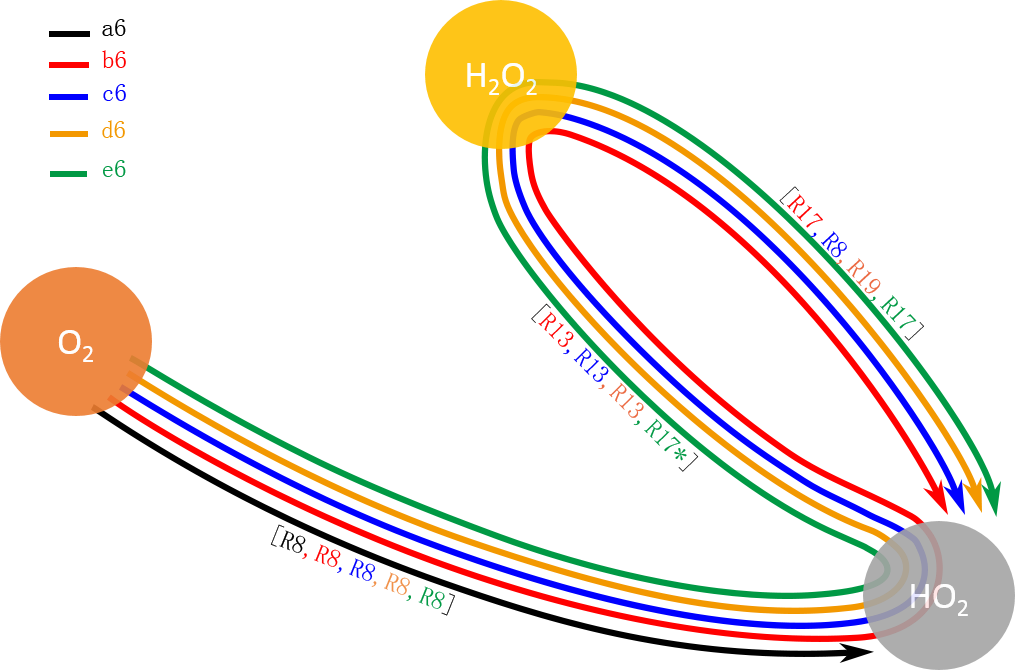
\includegraphics[width=100mm]{figs/chapter3/fig11.png}
    \end{center}
\label{ch3:fig11}
\end{figure}
\newline
\paragraph{}
It is seen that b6$-$e6 are cyclic paths. For all these pathways,
the HO$_2$ radical is first generated by recombination but then
reacts to form other species, such as H$_2$O$_2$, only then to
regenerate the HO$_2$ radical. These pathways are depicted in graphical form in Fig. \ref{ch3:fig11}. Because we are using O atom
following, the origin of the H atom in these pathways is not specified. Obviously, the formation of H radicals does involve
important rate limiting behavior for the formation of HO$_2$.

\section{Pathway Interpretation of Sensitivity}
\label{path_inter_s}
Now that the dominant pathways that lead to various species
targets have been uncovered, we can interpret the sensitivity
results presented in Fig. \ref{ch3:fig4} using the sum over histories
approach via $\tau = \sum_{i}{c_ip_i}$. Thus, each probability $p_i$ is a function of
$\mathbf{k}$ and has a total variance over the uncertainty range of $\sigma_{T}^{i,2}$. To
quantify the global sensitivity of the pathway probabilities with
respect to the individual rate coefficient $k_j$, we express each $p_i$ as
a first-order HDMR expansion, i.e.
\begin{equation}
\label{ch3:eqn18:tau_as_p}
p_i(k_1,k_2,\cdots,k_L) = p_{0}^{i} + \sum_{j=1}^{L}{F_j^i(k_j)}
\end{equation}
The component functions for pathway $i$, $F_j^i(k_j)$, were
expressed as fifth-order expansions in Legendre polynomials
fit using linear regression from 2000 sets of rate coefficients that
were randomly selected from the uncertainty range. We have
verified by direct computation that the totality of the second order
terms of the HDMR were small, typically on the scale of $\sim 5\%$ of the first-order terms, although they are occasionally
larger. We have also verified that there was not over-fitting of
the first-order component functions. We determine the first order
global sensitive coefficient for the pathway probability $p_i$ with respect to rate coefficient $k_j$ using the normalized partial variance
\begin{equation}
\label{ch3:eqn19:W_def}
\begin{split}
\widehat{W}_j^{i} &\equiv \frac{\sigma_j^{i,2}}{\sigma_T^{i,2}} \\
&= \frac{ \langle F_j^{i,2} \rangle }{\sigma_T^{i,2}}
\end{split}
\end{equation}
which is completely analogous to eqs \ref{ch3:eqn14} and \ref{ch3:eqn16:sigmaF}.
Correlations between pathways may be gauged using the coefficients
\begin{equation}
\label{ch3:eqn20_pcorr}
Corr(i,i\prime) = \frac{ \langle p_ip_{i\prime} \rangle - \langle p_i \rangle \langle p_{i\prime} \rangle  }{\sqrt{\sigma_T^{i,2}\sigma_T^{i\prime,2}}}
\end{equation}
If the first-order HDRM expansion, eqn. \ref{ch3:eqn18:tau_as_p}, is inserted into eqn. \ref{ch3:eqn20_pcorr}, it is seen that expressions of the following form appears.
\begin{equation}
\label{ch3:eqn21_W_i_j}
W_j^{i,i\prime} = \frac{\langle F_j^i F_j^{i\prime} \rangle}{\sigma_T^{i,2} \sigma_T^{i\prime,2}}
\end{equation}
The total correlation between paths $i$ and $i\prime$ may thus be
decomposed into contributions from the individual rate coefficients as
\begin{equation}
\label{ch3:eqn22_C_W_i_j}
Corr(i,i\prime) = \sum_{j=1}^{L}{ {\widehat{W}}_{j}^{i,i\prime} }
\end{equation}
We should note that this pathway correlation, $Corr(i,i\prime)$,
reflects how the change in flux along path i affects the flux along
path $i\prime$; it is not a correlation between individual reaction steps
which would require a higher order HDMR expansion to model.
\newline
\paragraph{}
Although the general chemical flux in the reaction network
may depend on the rate coefficients in a complicated manner,
there are two scenarios that are particularly simple for
interpretation. In the first, a single chemical pathway dominates
the flux to the target function $X_n(t)$. Under these circumstances,
the rate limiting step (i.e., the slowest step) to the target, and
the fastest step away from the target may prove the most
sensitive. For simplicity of illustration, assume that reactions
along the path are described by pseudo-first-order kinetics with
constant decay rates and branching ratios. The rate limiting
step to the target $X_n(t)$ is modeled by a pseudo-first-order rate
law $K_J$·$X_J$ and the fastest decay channel for $S_n$ is described by
$K_n$·$X_n$. We therefore expect the speciation target function to
behave as
\begin{equation}
\label{ch3:eqn23_X}
X_n(t) \approx X_0 \cdot \frac{K_J}{K_n - K_J} \left[e^{-K_n t} - e^{-K_J t}  \right]
\end{equation}
where $X_0$ is a constant. This approximate expression applies at
times that are long compared to the transient rates along the
pathway. Clearly, the target will show strong sensitivity to the
rate limiting formation step and/or the dominate decay step
and only weak sensitivity to the other steps. Although this
result is not surprising, it does serve to emphasize the
connection between pathways and sensitivity. A different
scenario occurs for “pathway switching” in which a sensitive
rate coefficient causes the reactive flux to change paths.
Consider the case where the largest flux pathway splits into two
branches (labeled a and b) that subsequently flow to the target $X_n(t)$. If we again assume pseudo-first-order kinetics, we have
the branching ratios
\begin{equation}
\label{ch3:eqn24_branch}
\begin{split}
\Gamma_a &= \frac{k_a}{k_a+k_b} \\
\Gamma_b &= \frac{k_b}{k_a+k_b}
\end{split}
\end{equation}
where $k_a$ and $k_b$ are the conventional rate coefficients at the
branching step. Then the contribution to the target will be
roughly given by
\begin{equation}
\label{ch3:eqn25}
X_n(t) \approx c \left( \Gamma_a p_a + \Gamma_b p_b \right)
\end{equation}
where c is a constant and pa and $p_b$ are the probabilities for
paths a and b. Thus, we expect there to be a large sensitivity of
the target to $k_a$ and $k_b$ provided that $p_a$ and $p_b$ are significantly
different numerically. We also predict a high level of correlation
between the factors $k_a$ and $k_b$.
\newline
\paragraph{}
\begin{figure}[htbp]
	\caption[Sensitivity indices of the pathways leading to the H$_2$O target concentration]{Sensitivity indices of the pathways leading to the H$_2$O target concentration evaluated at $t=0.8\tau_{ign}$. In this figure we plot $F_j^{i,2}/\sigma_T^{i,2}$, where each path has a common normalizing factor so that less probable pathway show smaller indices.}
    \begin{center}
	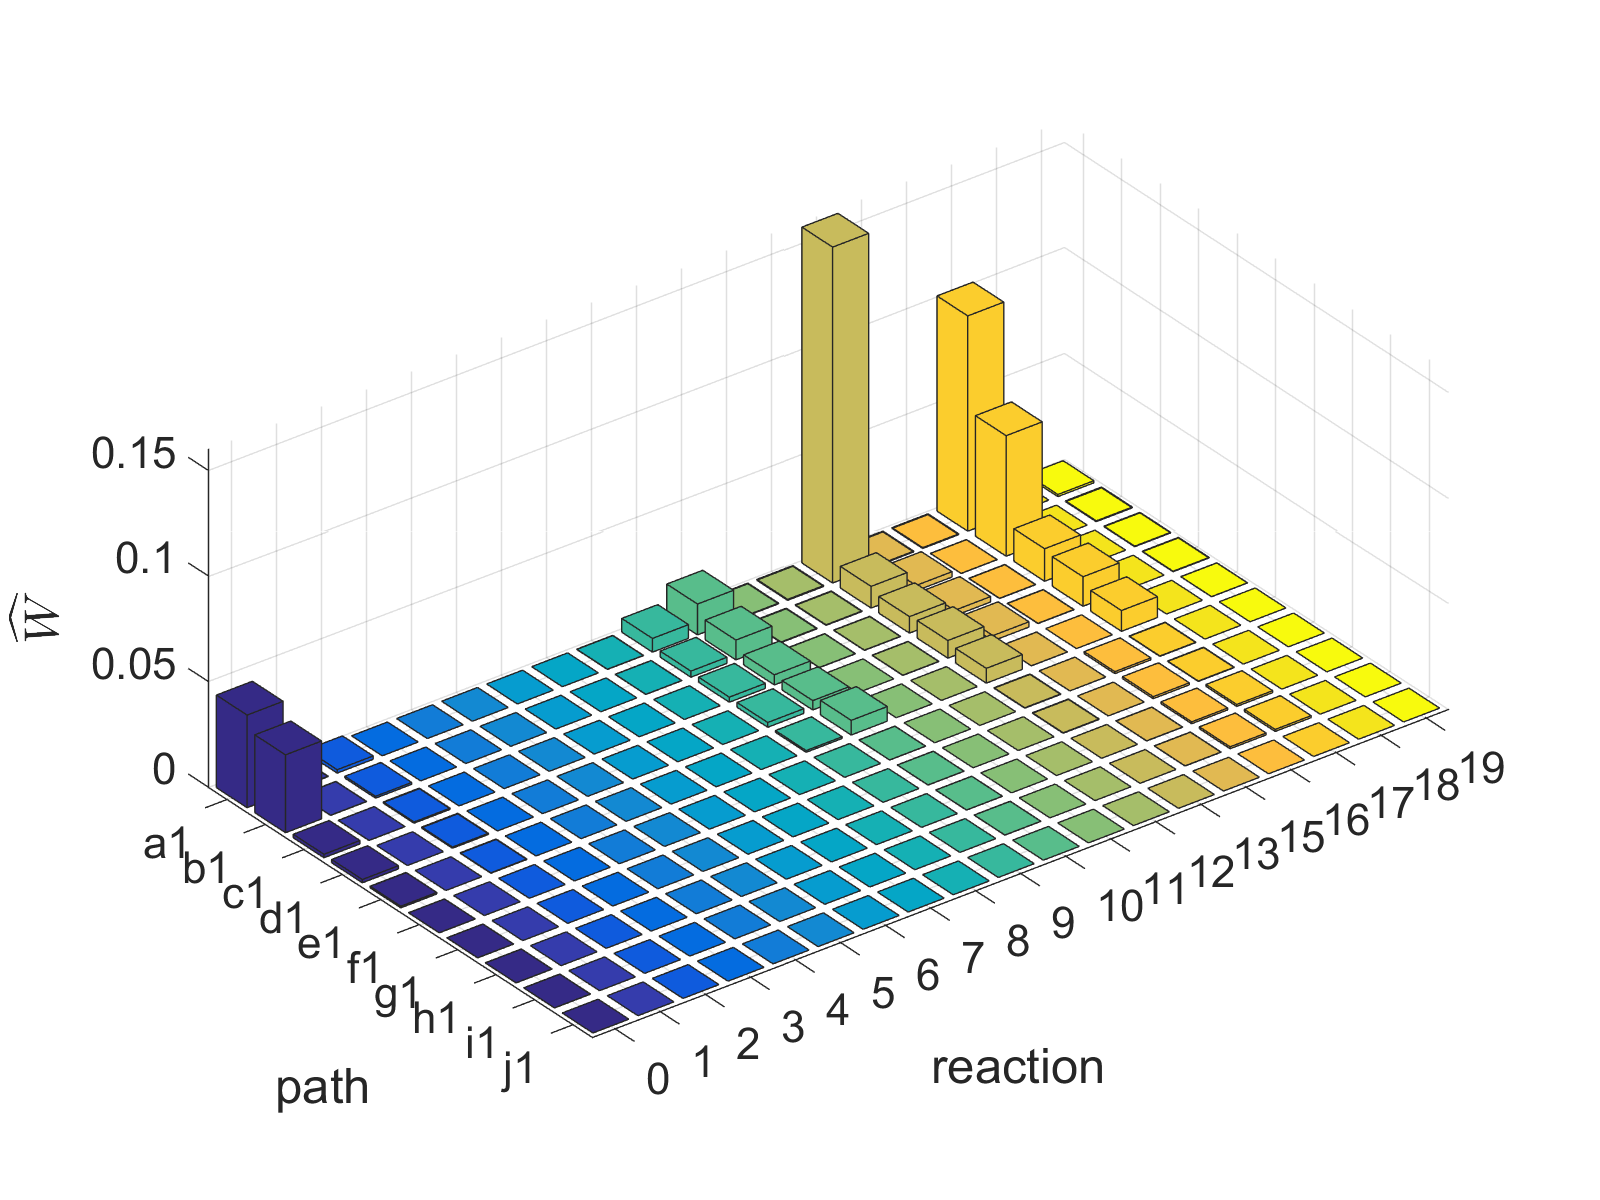
\includegraphics[width=100mm]{figs/chapter3/fig12.png}
    \end{center}
\label{ch3:fig12}
\end{figure}

\begin{figure}[htbp]
 \begin{subfigure}[b]{0.5\textwidth}
 \center{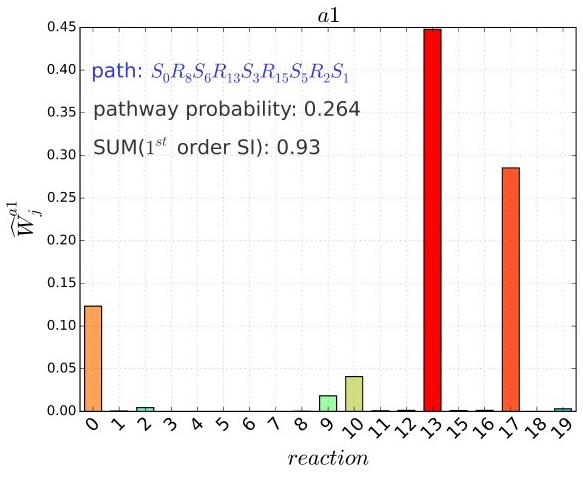
\includegraphics[width=\textwidth]{figs/chapter3/fig13_a.png}}
 \label{ch3:fig13a}
 \end{subfigure}
  \begin{subfigure}[b]{0.5\textwidth}
 \center{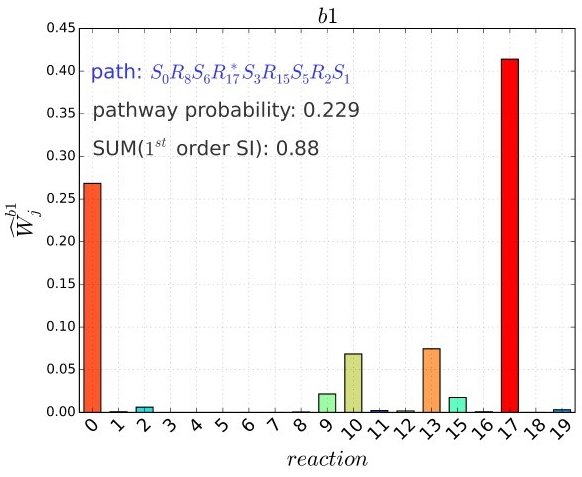
\includegraphics[width=\textwidth]{figs/chapter3/fig13_b.png}}
 \label{ch3:fig13b}
  \end{subfigure}
  \begin{subfigure}[b]{0.5\textwidth}
 \center{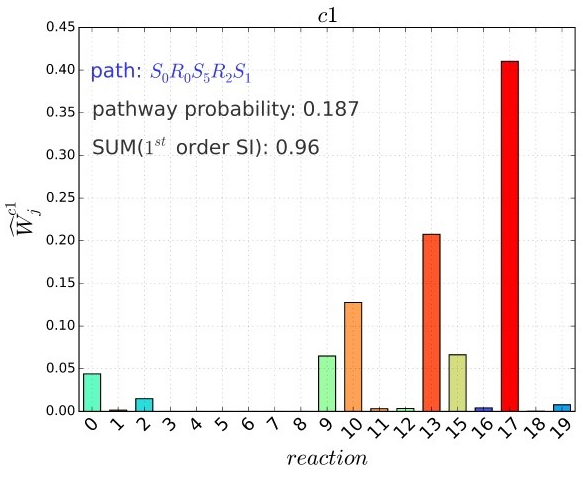
\includegraphics[width=\textwidth]{figs/chapter3/fig13_c.png}}
 \label{ch3:fig13c}
 \end{subfigure}
  \begin{subfigure}[b]{0.5\textwidth}
 \center{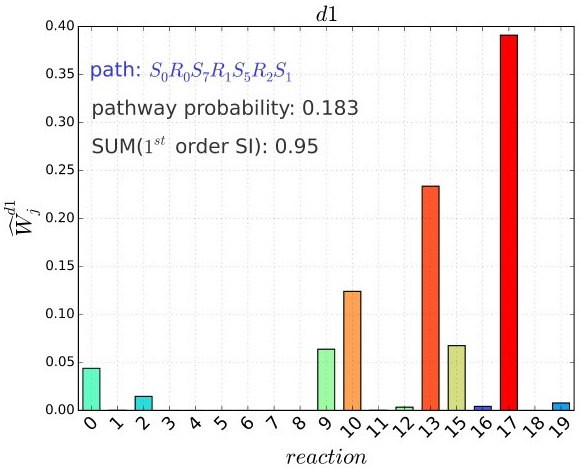
\includegraphics[width=\textwidth]{figs/chapter3/fig13_d.png}}
 \label{ch3:fig13d}
 \end{subfigure}
 \begin{subfigure}{0.5\textwidth}
 \center{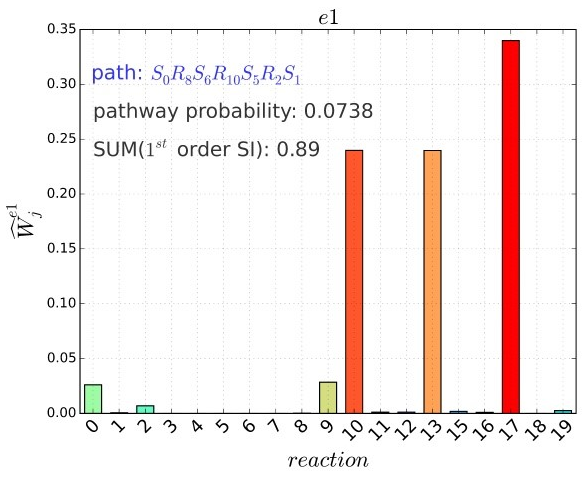
\includegraphics[width=\textwidth]{figs/chapter3/fig13_e.png}}
 \label{ch3:fig13e}
 \end{subfigure}
 \caption[Sensitivity indices for the five most important paths leading to the H$_2$O target]{Sensitivity indices versus reaction index for the five most important paths leading to the H$_2$O target evaluated at time $0.8\tau_{ign}$. The relevant reactions for each path are reproduced on the figure panels. Also shown in each panel is the pathway probability and the sum of first-order indices obtained by the HDMR expansion of $p_i$.}
\label{ch3:fig13}
\end{figure}


As an application, consider the $\left[ H_2O \right]$ target, which
possesses the most interesting and complicated pathway
representation. We focus first on a single time, $t=0.8\tau_{ign}$.
From the global sensitivity results of Fig. \ref{ch3:fig4}, we see that the
most important reactions for the H$_2$O formation at this time
are, in descending order, R13, R0, R17, R9, and R10. We can
understand this pattern from the behavior of the paths. At $t=0.8\tau_{ign}$, the pathway probabilities are 0.264 (a1), 0.229 (b1),
0.187 (c1), 0.184 (d1), and 0.074 (e1). In Fig. \ref{ch3:fig12} we show the spectrum of sensitivity indices, i.e.,$\widehat{W}_j^{1}$ versus $j$, obtained for the largest pathways ranked by order of probability. In this
figure, we have plotted sensitivity indices using a common normalization factor, i.e., $ \langle F_j^{i,2} \rangle / \sigma_T{2}$ where $\sigma_T^2$ is the total variance
for all paths, so that that the less important pathways show
lower indices. In Fig. \ref{ch3:fig13} we show the sensitivity spectrum for
the five most probable paths, a1\-e1, using the conventional
normalization, eqn. \ref{ch3:eqn19:W_def}. First, we note that the reactions that have
the largest value of H$_2$O target sensitivity, $W_j$, in Fig. \ref{ch3:fig4} are
also, on average, the most sensitive reactions for the paths
leading to the target. However, we notice that the detailed
distributions of ${\widehat{W}}_j^{1}$ values differ significantly from pathway to
pathway. For brevity we use the pathway superscript $i$ going
from 1$-$5 for pathways a1$-$e1. The most probable path, a1,
shows strongest sensitivity to R13 and R17 with a modest
contribution from R0, i.e., ${\widehat{W}}_{13}^{1} > {\widehat{W}}_{17}^{1} > {\widehat{W}}_{0}^{1}$. For the second
most important path, b1, the contribution from R17 is now
clearly the largest, with R2 second and R13 and R10 also present, i.e., ${\widehat{W}}_{17}^{2} > {\widehat{W}}_{2}^{2} > {\widehat{W}}_{13}^{2} \approx {\widehat{W}}_{10}^{2}$. Paths c1 and d1 give a
nearly identical spectrum because, as discussed in section \ref{Description_of_Chemical_Pathway},
they are closely related physically. For those two paths, we see that ${\widehat{W}}_{17}^{3} > {\widehat{W}}_{13}^{3} > {\widehat{W}}_{10}^{3}$. For e1, we have ${\widehat{W}}_{17}^{5} > {\widehat{W}}_{13}^{5} \approx {\widehat{W}}_{10}^{5}$. We can understand the results of Fig. \ref{ch3:fig13} from the detailed
character of the chemical pathways. The pathway a1 is most
sensitive to R13, which is rate limiting along this pathway. For
b1, on the contrary, the reaction R17* is most sensitive because it is rate limiting for this pathway. We note that both ${\widehat{W}}_{17}^{3}$ and ${\widehat{W}}_{13}^{3}$ are appreciable in both the a1 and b1 spectra due to the
pathway switching mechanism. Clearly, by changing the ratio
$k_{13}/k_{17}^{\ast}$, we will alter whether the O atom follows the a1 path
or the b1 path. Indeed, inspection of the graph in Fig. \ref{ch3:fig8}
shows that a1 and b1 are identical except for the step where the
HO2 radical decays via $\text{H}\textcolor{red}{\textbf{O}}_2 (+\text{HO}_2) \xrightarrow[\text{R}_{13}]{\makebox[1cm]{}} \text{H}_2\textcolor{red}{\textbf{O}}_2$ for a1 and
via $\text{H}\textcolor{red}{\textbf{O}}_2 (+\text{H}_2) \xrightarrow[\text{R}_{17}^{*}]{\makebox[1cm]{}} \text{H}_2\textcolor{red}{\textbf{O}}_2$ for b1. It is interesting to notice
that R0, H + O$_2$ $\rightarrow$ OH + O, is quite important for a1 and b1
even though this step does not enter into either path. More
understandably, this reaction is also sensitive in c1 and d1,
where it is the initial step. For a1 and b1, the graphs in Figs.
\ref{ch3:fig5} and \ref{ch3:fig9} make it is easy to see that R0 is in competition with R8,
H + O$_2$ + M $\rightarrow$ HO$_2$ + M, which is the initial step for a1 and
b1. Thus, again the sensitivity to R0 is a case of pathway
switching between (c1, d1) and (a1, b1). The pathway e1 is
interesting in that the reaction R10, HO$_2$ + H $\rightarrow$ OH + OH,
emerged as the key step. This is consistent with the observation
that the sensitivity index ${\widehat{W}}_{10}^{5}$ for this reaction is seen to be
quite large. That R13 and R17$^{\ast}$ are also sensitive reactions
again reflects the competition from those reactions for the HO$_2$
radical and thus pathway switching.
\newline
\paragraph{}
In addition to the sensitivity indices of the pathway
probabilities, we have also computed the correlations between
the pathways that lead to the H$_2$O target. In the interest of
brevity, we focus on the correlation that develops within just
two pairs of pathways, (a1, b1) and (a1, c1). Using eqn. (\ref{ch3:eqn21_W_i_j}), we
see in Fig. \ref{ch3:fig14} that the largest interactions for the (a1, b1)
pair, ${\widehat{W}}_j^{a1,b1}$, are due to reaction R17$^\ast$, a negative correlation,
and reactions R0 and R13, positive correlations. For the (a1, c1) pair, ${\widehat{W}}_{17}^{a1,c1}$, is again the largest, with a positive ${\widehat{W}}_{13}^{a1,c1}$, the
next largest but ${\widehat{W}}_0^{a1,c1}$ now yielding a negative correlation. The
explanation for these results can be provided by examining the
first-order component functions, $F_j^ i (k_j)$, for paths i = a1, b1, c1.
In Fig. \ref{ch3:fig15} we plot $F_j^ i (k_j)$ for a1, b1, and c1 over the
uncertainty range for each rate coefficient. Note that ⟨$F_j^ i (k_j)$⟩ =
0 because the mean probability is already taken out. The negative correlation for reaction R17$^{\ast}$ arises because $F_{17}^{a1}(k_{17}^{\ast})$ decreases with increasing k17$^\ast$ whereas $F_{17}^{b1}(k_{17}^{\ast})$ and $F_{17}^{c1}(k_{17}^{\ast})$ both increase. This is quite understandable because for path a1
reactions R13 and R17$^{\ast}$ are in competition to consume the
HO$_2$ radical; thus an increase in k17$^\ast$ decreases the flux along
path a1 for which the R13 step is rate limiting. On the contrary,
pathway b1 includes the rate limiting R17$^\ast$ step and so
increasing k17$^\ast$ promotes this pathway. The pathway probability
for c1 (i = 2) increases with k17$^\ast$ because reaction R17$^\ast$
produces an H-radical which then promotes reaction R0, H +
O$_2$ $\rightarrow$ OH + O. Because reaction R13 leads to the formation of
H$_2$O$_2$, which almost always decays to OH + OH, increasing k13
also increases the probability for c1 by promoting reaction R2,
OH + H$_2$ $\rightarrow$ H$_2$O + H. Finally, $F_{0}^{2}(k_0)$ increases with increasing
k0 because R0 is the initiation step of this pathway; on the contrary, $F_{0}^{0}(k_0)$ and $F_{0}^{1}(k_0)$ both decrease with increasing k0 because R0 is in competition with R8, which initiates pathways
a1 and b1. In a similar fashion we could also understand the
correlations that develop between other pathways in the model.
\begin{figure}[htbp]
	\caption[Correlation between pathways]{Correlation between pathways (a1, b1) in the upper panel and (a1, c1) in the lower panel for the H2O target evaluated at $t=0.8\tau_{ign}$. The correlation has been decomposed into the contributions
from specific reactions via eqn. \ref{ch3:eqn21_W_i_j}.}
    \begin{center}
	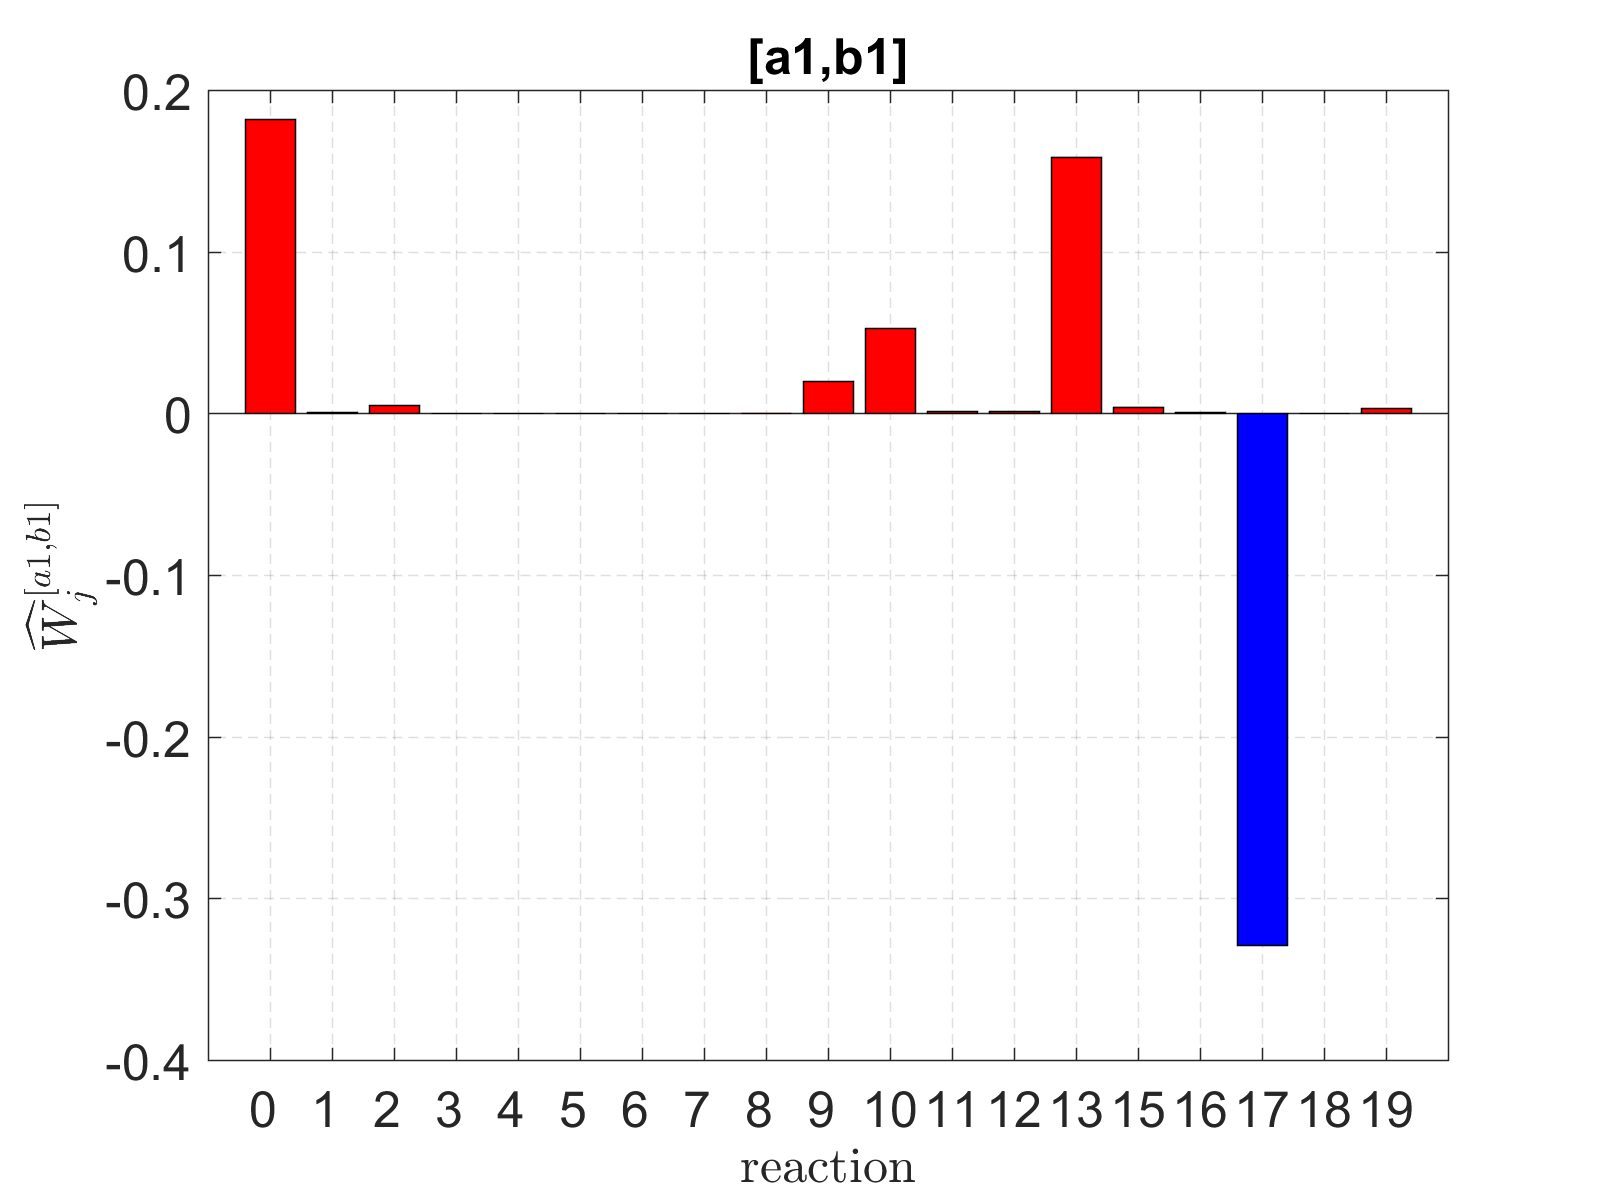
\includegraphics[width=100mm]{figs/chapter3/fig14_1.png}
    \end{center}
\label{ch3:fig14}
\end{figure}
\begin{figure*}[htbp]
    \begin{center}
	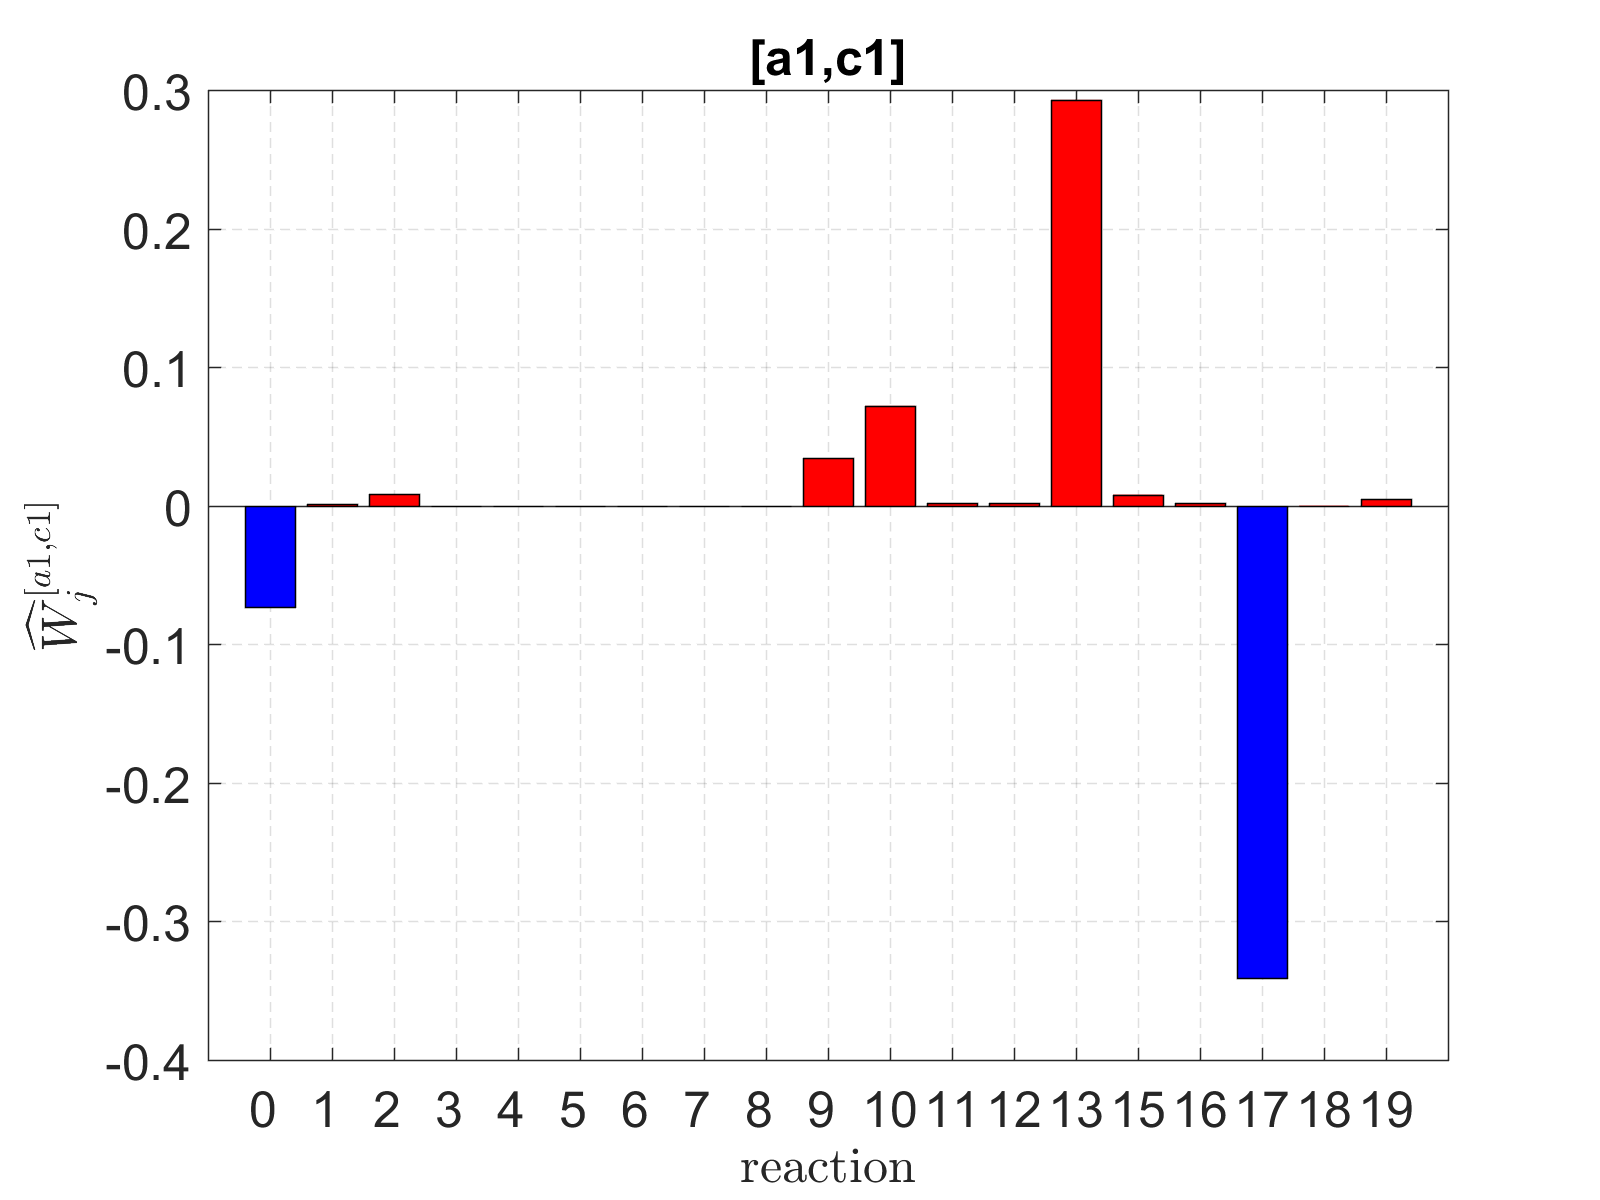
\includegraphics[width=100mm]{figs/chapter3/fig14_2.png}
    \end{center}
\end{figure*}
\begin{figure}[htbp]
	\caption[1$^{st}$ order component function of the pathway probabilities a1, b1, and c1]{First-order component function for the HDMR expansion
of the pathway probabilities a1, b1, and c1 for the H$_2$O target
evaluated at $t=0.8\tau_{ign}$.}
    \begin{center}
	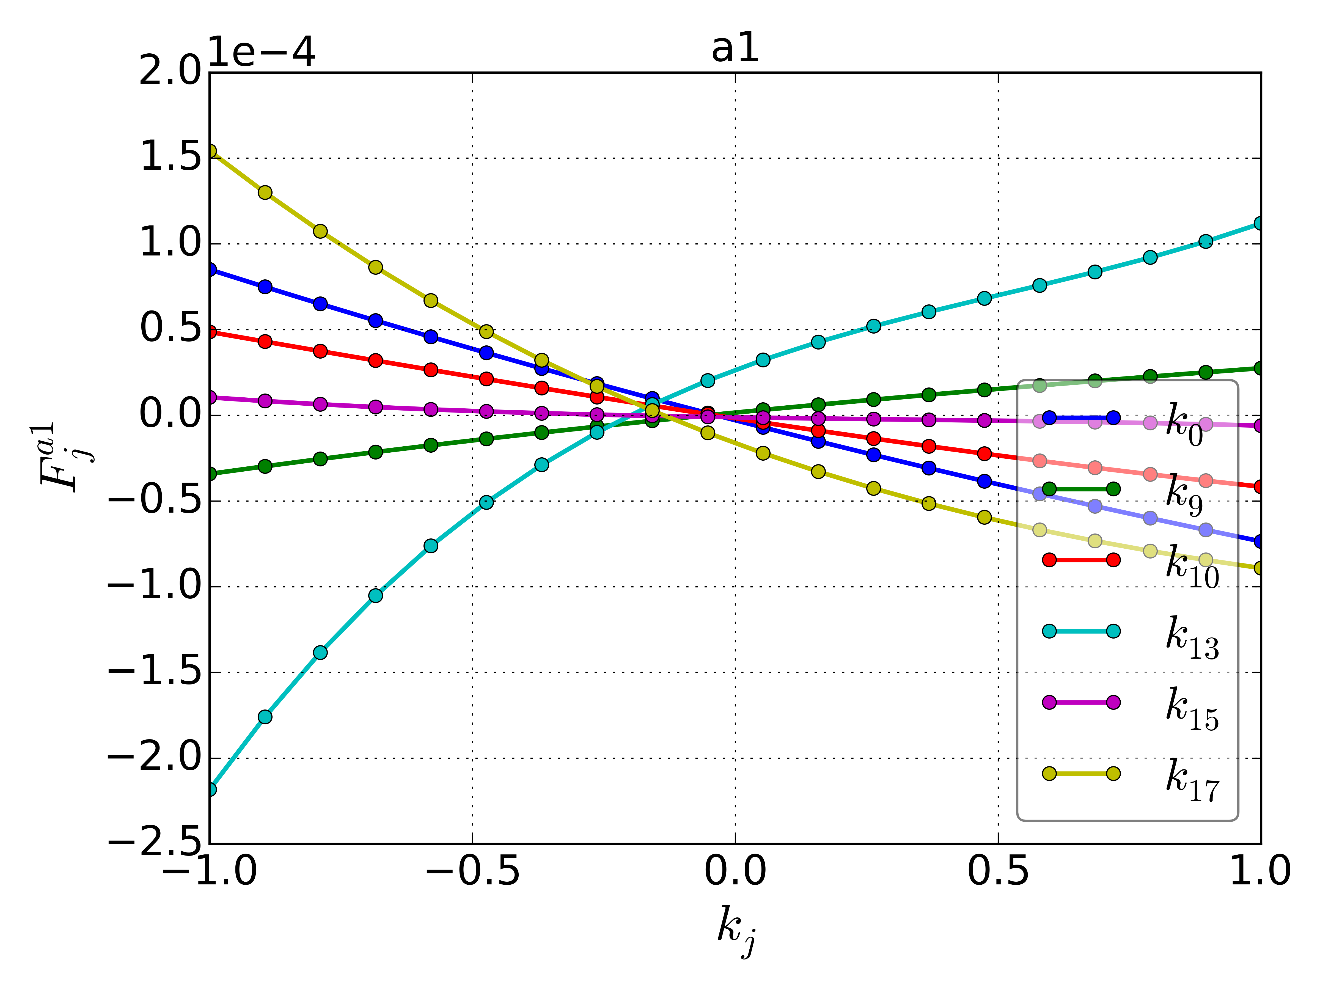
\includegraphics[width=100mm]{figs/chapter3/fig15_a.png}
    \end{center}
\label{ch3:fig15}
\end{figure}
\begin{figure*}[htbp]
    \begin{center}
	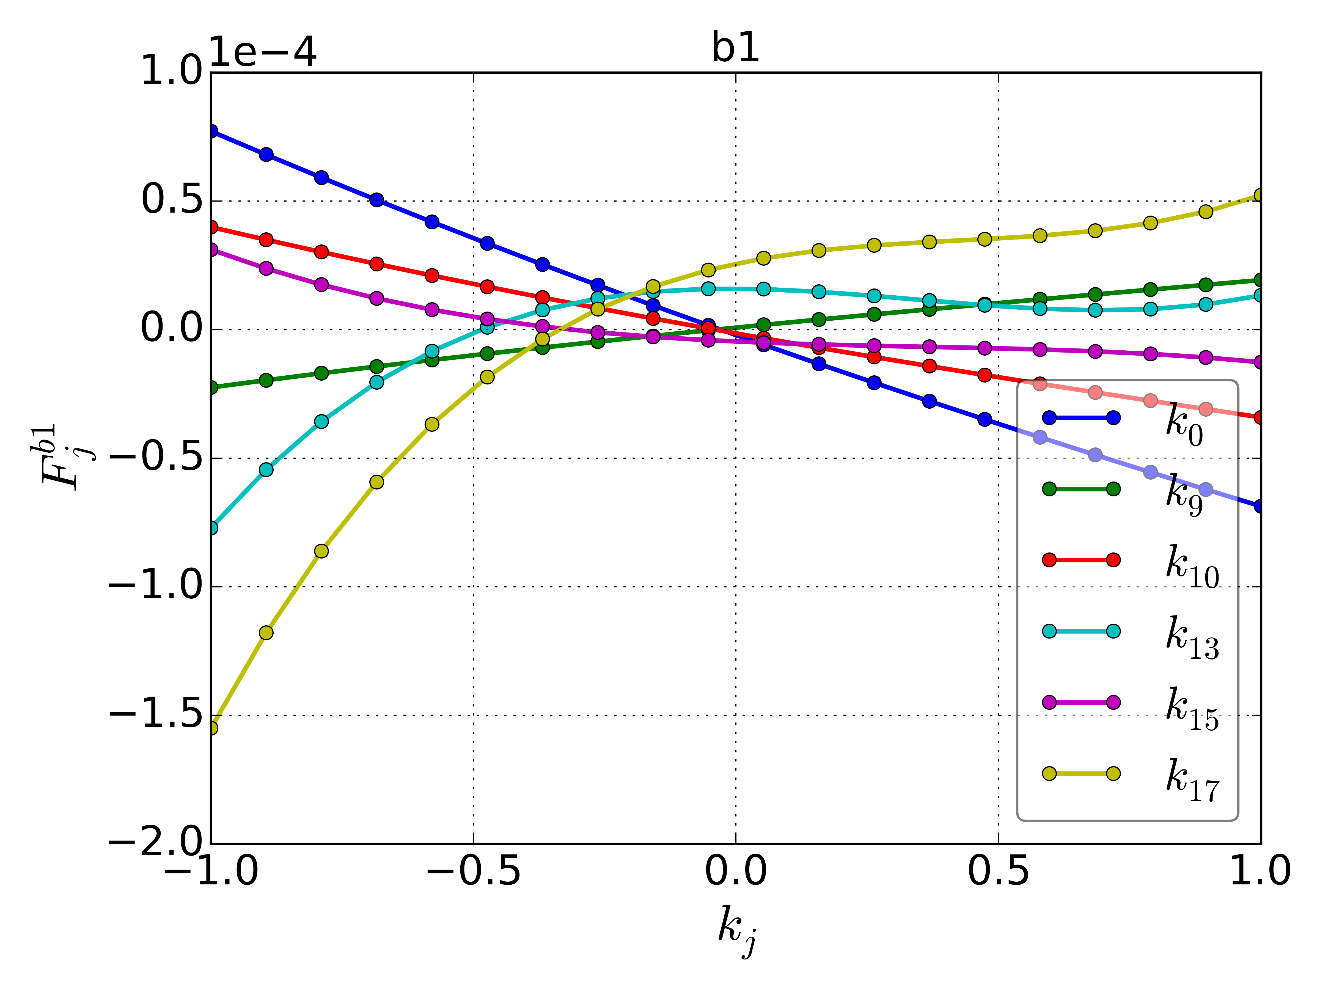
\includegraphics[width=100mm]{figs/chapter3/fig15_b.png}
    \end{center}
\end{figure*}
\begin{figure*}[htbp]
    \begin{center}
	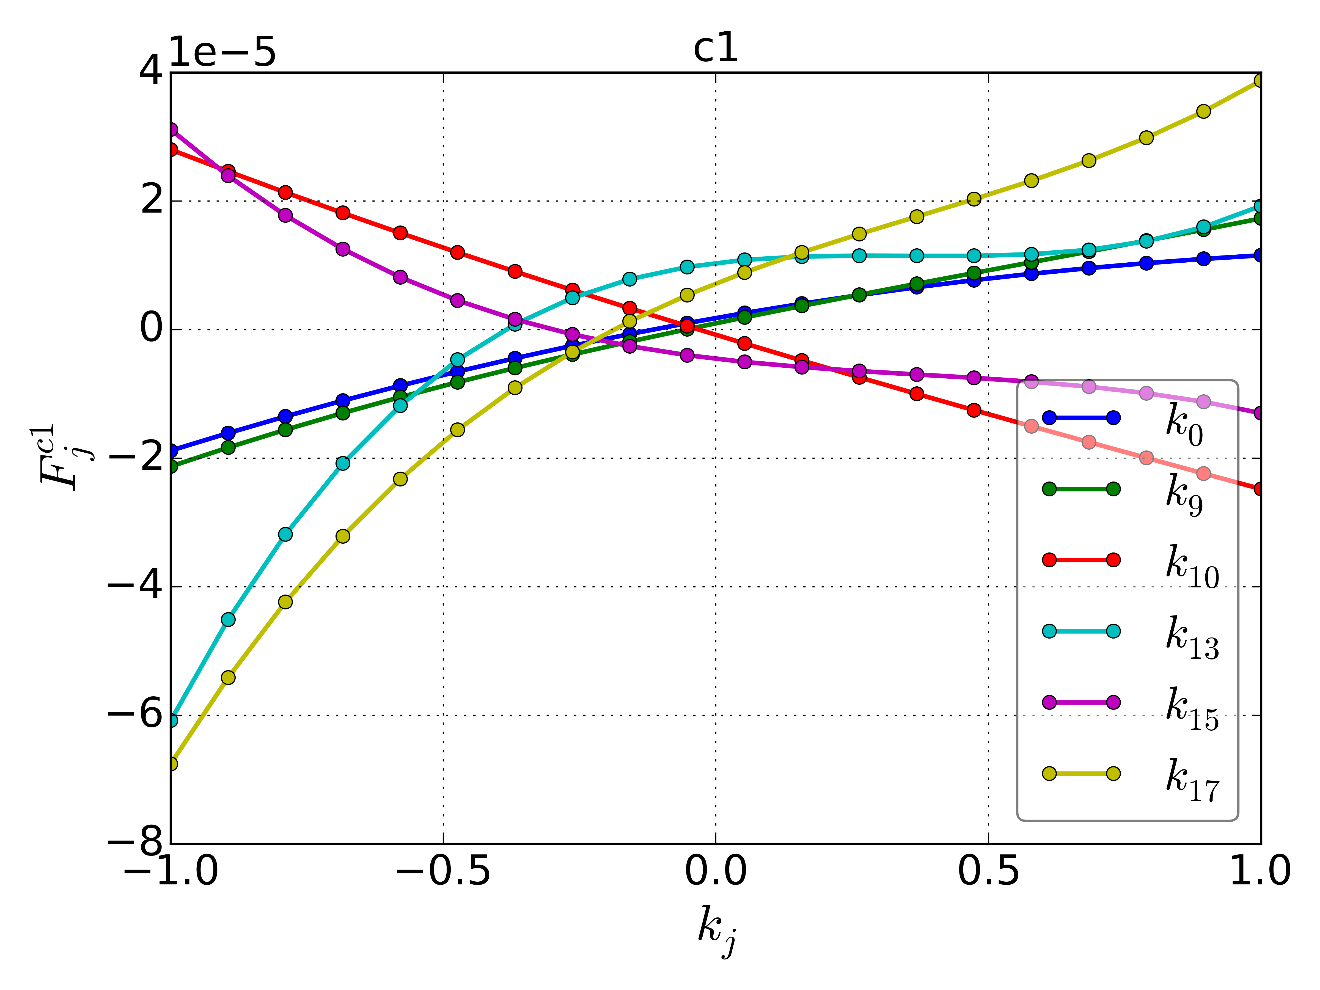
\includegraphics[width=100mm]{figs/chapter3/fig15_c.png}
    \end{center}
\end{figure*}
\paragraph{}
\newline
\paragraph{}
One of the most interesting aspects of the H$_2-$O$_2$ system is
the crossover behavior where the R17$^{\ast}$ is the main source of
H$_2$O$_2$ at early times whereas R13 becomes largest at long times.
This mechanistic crossover is apparent in the overall reaction
rates, Fig. \ref{ch3:fig2}, which shows that the rate for R13 crosses and
then exceeds that for R17$^{\ast}$ at about $t=0.5\tau_{ign}$. In terms of pathways, H$_2$O$_2$ production is dominated by just two, a3 and b3, which account for over $99\%$ of the total. These two paths
differ only in the step that produces H$_2$O$_2$ from HO$_2$, reactions
R13 and R17$^{\ast}$, respectively. Thus, in Fig. \ref{ch3:fig6}, we saw that the
pathway probability for a3 likewise crosses and exceeds that for
b3 at roughly the same point in time as the rates. It is
instructive to study the pathway sensitivities versus time for this
crossover regime. In Fig. \ref{ch3:fig16} we see the sensitivities for paths
a3 and b3 are dominated by R13 and R17$^{\ast}$, respectively, but in
a quite asymmetrical way. As we might expect, pathway a3 is
more sensitive to R13 than to R17$^{\ast}$ and b3 is more sensitive to
R17$^{\ast}$ than R13. However, the degree of sensitivity and the
shapes of the profiles versus time are dissimilar, which reflects
the differing functional dependence of $p_{a3}$ and $p_{b3}$ on the rate
coefficients. The a3 pathway shows a growth in both the R13
and R17$^{\ast}$ sensitivity near the $t=0.5\tau_{ign}$ crossover point. The b3
pathway shows a significant growth in R17$^{\ast}$ sensitivity early in
the ignition process and a more complicated oscillating
sensitivity to R13 versus time.
\begin{figure}[htbp]
	\caption[Sensitivity indices for the two dominant paths leading to
H$_2$O$_2$]{Sensitivity indices for the two dominant paths leading to
H$_2$O$_2$ as a function of time.}
    \begin{center}
	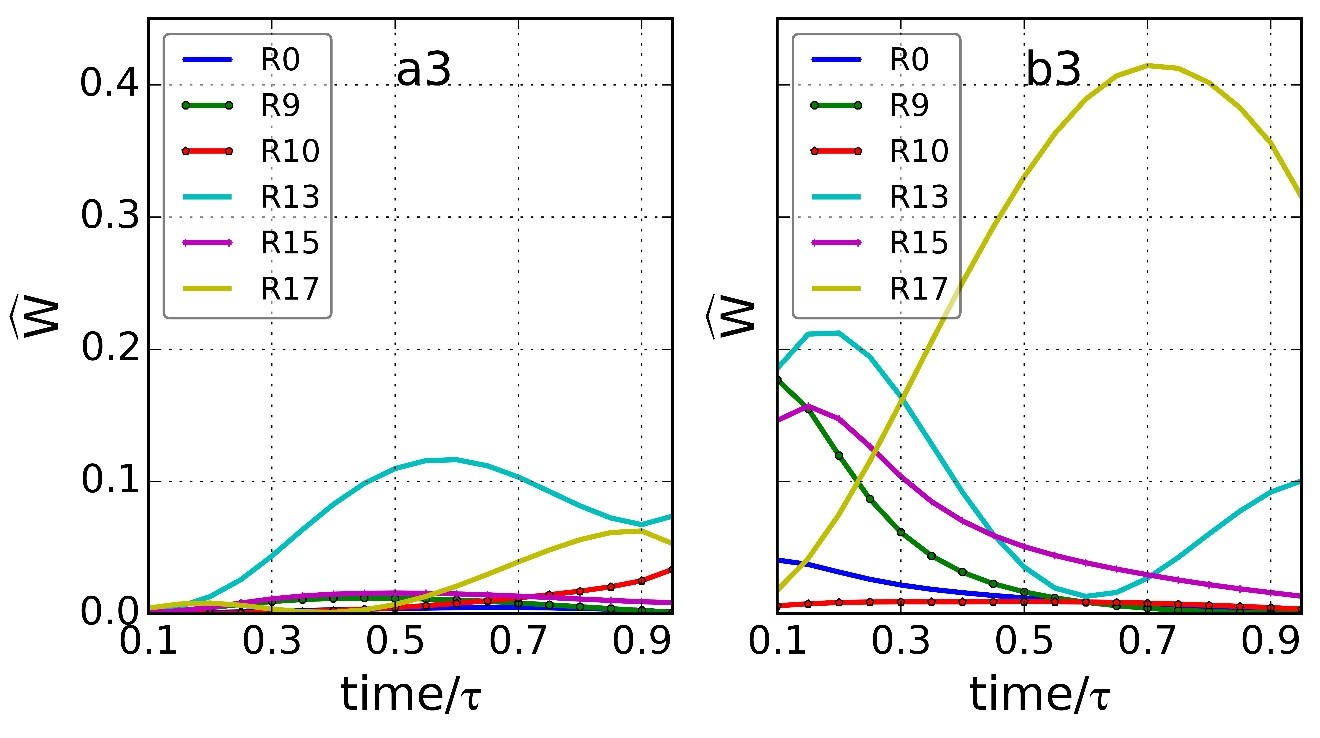
\includegraphics[width=100mm]{figs/chapter3/fig16.jpg}
    \end{center}
\label{ch3:fig16}
\end{figure}
\newline
\paragraph{}
Finally, we note the unexpected results obtained for the HO$_2$
target. The sensitivity indicies for this target shown in Fig. \ref{ch3:fig4}
are generally similar to that for other species, viz. strong
contributions from the R13, R17$^{\ast}$, R15, and R9. Unlike the
other species, however, HO$_2$ formation is dominated by a single
one-step chemical pathway, O$_2$ + H + M $\rightarrow$ HO$_2$ + M,
described by R8. Hence, it is at first surprising that R8 does not
significantly contribute to the sensitivity spectrum at any time.
Instead, the $W_j$ are largest for reactions involved in the decay of the HO$_2$ species, R13 and R17$^{\ast}$, and the secondary decay of
H$_2$O$_2$, i.e., R15. The lack of R8 dependence is partly due to use
of O atom following. Clearly, HO$_2$ formation is limited not by
oxygen but instead by the formation of H-radicals. Indeed, R8 is
found to be much faster that R17$^{\ast}$ (HO$_2$ + H$_2$ $\rightarrow$ H + H$_2$O$_2$)
and R9 (H$_2$ + O$_2$ $\rightarrow$ HO$_2$ + H), which are both sources of H
atoms and both appear in the sensitivity spectrum.

\section{Conclusions}
\label{conclusions}
The sum over histories approach offers a uniquely quantitative
method for investigating the contribution of distinct and
competing chemical pathways to the behavior of large
mechanisms. The sum over histories method allows the
concentration of species to be represented in terms of a sum over the probabilities for chemical pathways that generate that
species. This method differs from other techniques for reaction
path analysis that represent the pathways at an instant of time
using a flux snapshot. Instead, our method permits the time
evolving chemistry of the system to be quantitatively
incorporated into the probability for the chemical pathways.
Hence, the dominant chemical pathways followed by chemical
moieties are allowed to change as time progresses. In the
present work we have used the sum over histories approach to
analyze the sensitivity of speciation in the H$_2-$O$_2$ combustion
system. Thus, the formation of any target species is described in
terms of a sequence of reactions that carry a tagged atom from
reactants to the target. Using O atom following, it was found
that a small number of chemical pathways could account for the
formation of the products and intermediates prior to the
ignition time. The observed sensitivities for species targets to
the values of the rate coefficients could, for the most part, be
traced to key steps along the chemical pathways. In particular, it
was observed that the chemistry of HO$_2$ radicals and the
subsequent formation of H$_2$O$_2$ were essential steps along many
dominate chemical pathways. It was found that high sensitivity
was often associated with rate limiting steps or pathway
switching phenomena involving HO$_2$ self-reaction, R13, and
HO$_2$ + H$_2$, R17$^{\ast}$.
\newline
\paragraph{}
As a final point, we note that there remains an element of
choice when applying the sum over histories representation,
specifically in the selection of the chemical moiety to be
followed. In principle, we may select any atom in the target
molecule as our followed atom to implement the algorithm.
However, the efficiency of the method, and the insight it
affords, does depend on this choice. For the present H$_2-$O$_2$
combustion problem, e.g., we found that O atom following
procedure was more rapidly convergent and more useful for
interpretation than the H atom following approach. However,
the sensitivity of HO$_2$ species formation to the rate coefficients
could not be well explained in this representation. Instead, the
formation of HO$_2$ is largely controlled by H atom production
required for the association reaction H + O$_2$ + M $\rightarrow$ HO$_2$ + M.
Hence, for this species it is advisable to switch to the H atom
following scheme to understand the results of the sensitivity
analysis.